\chapter{Konzeption des Metamodells}

\section{Konzeptionelle Rahmenbedingungen}

\subsection{Einleitende Überlegungen}

Folgende Voraussetzungen werden für diese modellgetriebene Entwicklung festgelegt: Das zu entwerfende Metamodell soll die Konzepte von Microservice-Architekturen aufgreifen. Dabei soll die noch zu definierende Auswahl der Technologien, die für eine Umsetzung benötigt werden, berücksichtigt werden. Auch die Möglichkeit, andere Technologien verwenden zu können, soll bedacht werden. Weiterhin wird davon ausgegangen, dass zusätzliche Software zum Betrieb einer Microservice-Architektur vorhanden ist. Kandidaten für solche Software wären die Cloud-Umgebung, die Datenbanktechnologie oder Software Development Kits. Die vorausgesetzte Software muss daher definiert und berücksichtigt werden. Ebenso wird die Einbindung von grafischen Oberflächen für die entwickelten Microservices in der Konzeption nicht betrachtet. Zu konzipieren ist hingegen eine Umsetzung durch APIs, welche ein von dieser Modellierung unabhängiges Frontend beliefern könnten.

Methodisch soll zu Beginn der State of the Art erfasst und in einen Kontext zur Zielstellung dieser Arbeit gesetzt werden. Dabei sollen Möglichkeiten zum Einbezug bestehender Forschungsergebnisse geprüft werden. Die Abstraktion soll in ihrem Vorgehen auf den theoretischen Grundlagen von Microservice-Architekturen beruhen. Abweichungen von diesen sollen nach Möglichkeit vermieden werden. Die zu entwerfende abstrakte Syntax soll iterativ im Kontext der Darstellung und Generierung verbessert werden. Grund dafür ist die frühe Erkennung von konzeptionellen Fehlern und Problemen. Diese sollen dabei gelöst werden und bei der Erklärung des schließlich entstehenden Metamodells angesprochen werden. Auf eine Visualisierung dieser Zwischenlösungen wird verzichtet. Der anwendungsorientierte Teil der Entwicklung soll einerseits lokal und in einer Cloud-Umgebung durchgeführt werden.

Für die Entscheidungsfindung und die abschließende Bewertung der Konzeption werden folgende Kriterien festgelegt: Das Hauptkriterium ist der Mehrwert, den die Generierung von Anwendungen für Cloud-Umgebungen bietet, insbesondere in Bezug auf die Lösung realer Probleme. Zusätzlich soll die Entwicklung kritisch auf die Einbindung von Eigenschaften und Konzepten von Microservices geprüft werden. Es gilt bei dem Entwurf der abstrakten Syntax auch, die Erweiterbarkeit dieser zu ermöglichen. Weitere Kriterien sind das mögliche Potential für Code-Wiederverwendung, die Möglichkeit, durch Abstraktion und Visualisierung Komplexität greifbarer zu machen, und die Nutzung im Rahmen von Refaktorisierungen.

\subsection{Einbindung aktueller Technologien}

\subsubsection{AjiL}

\begin{figure}[ht]
\centering
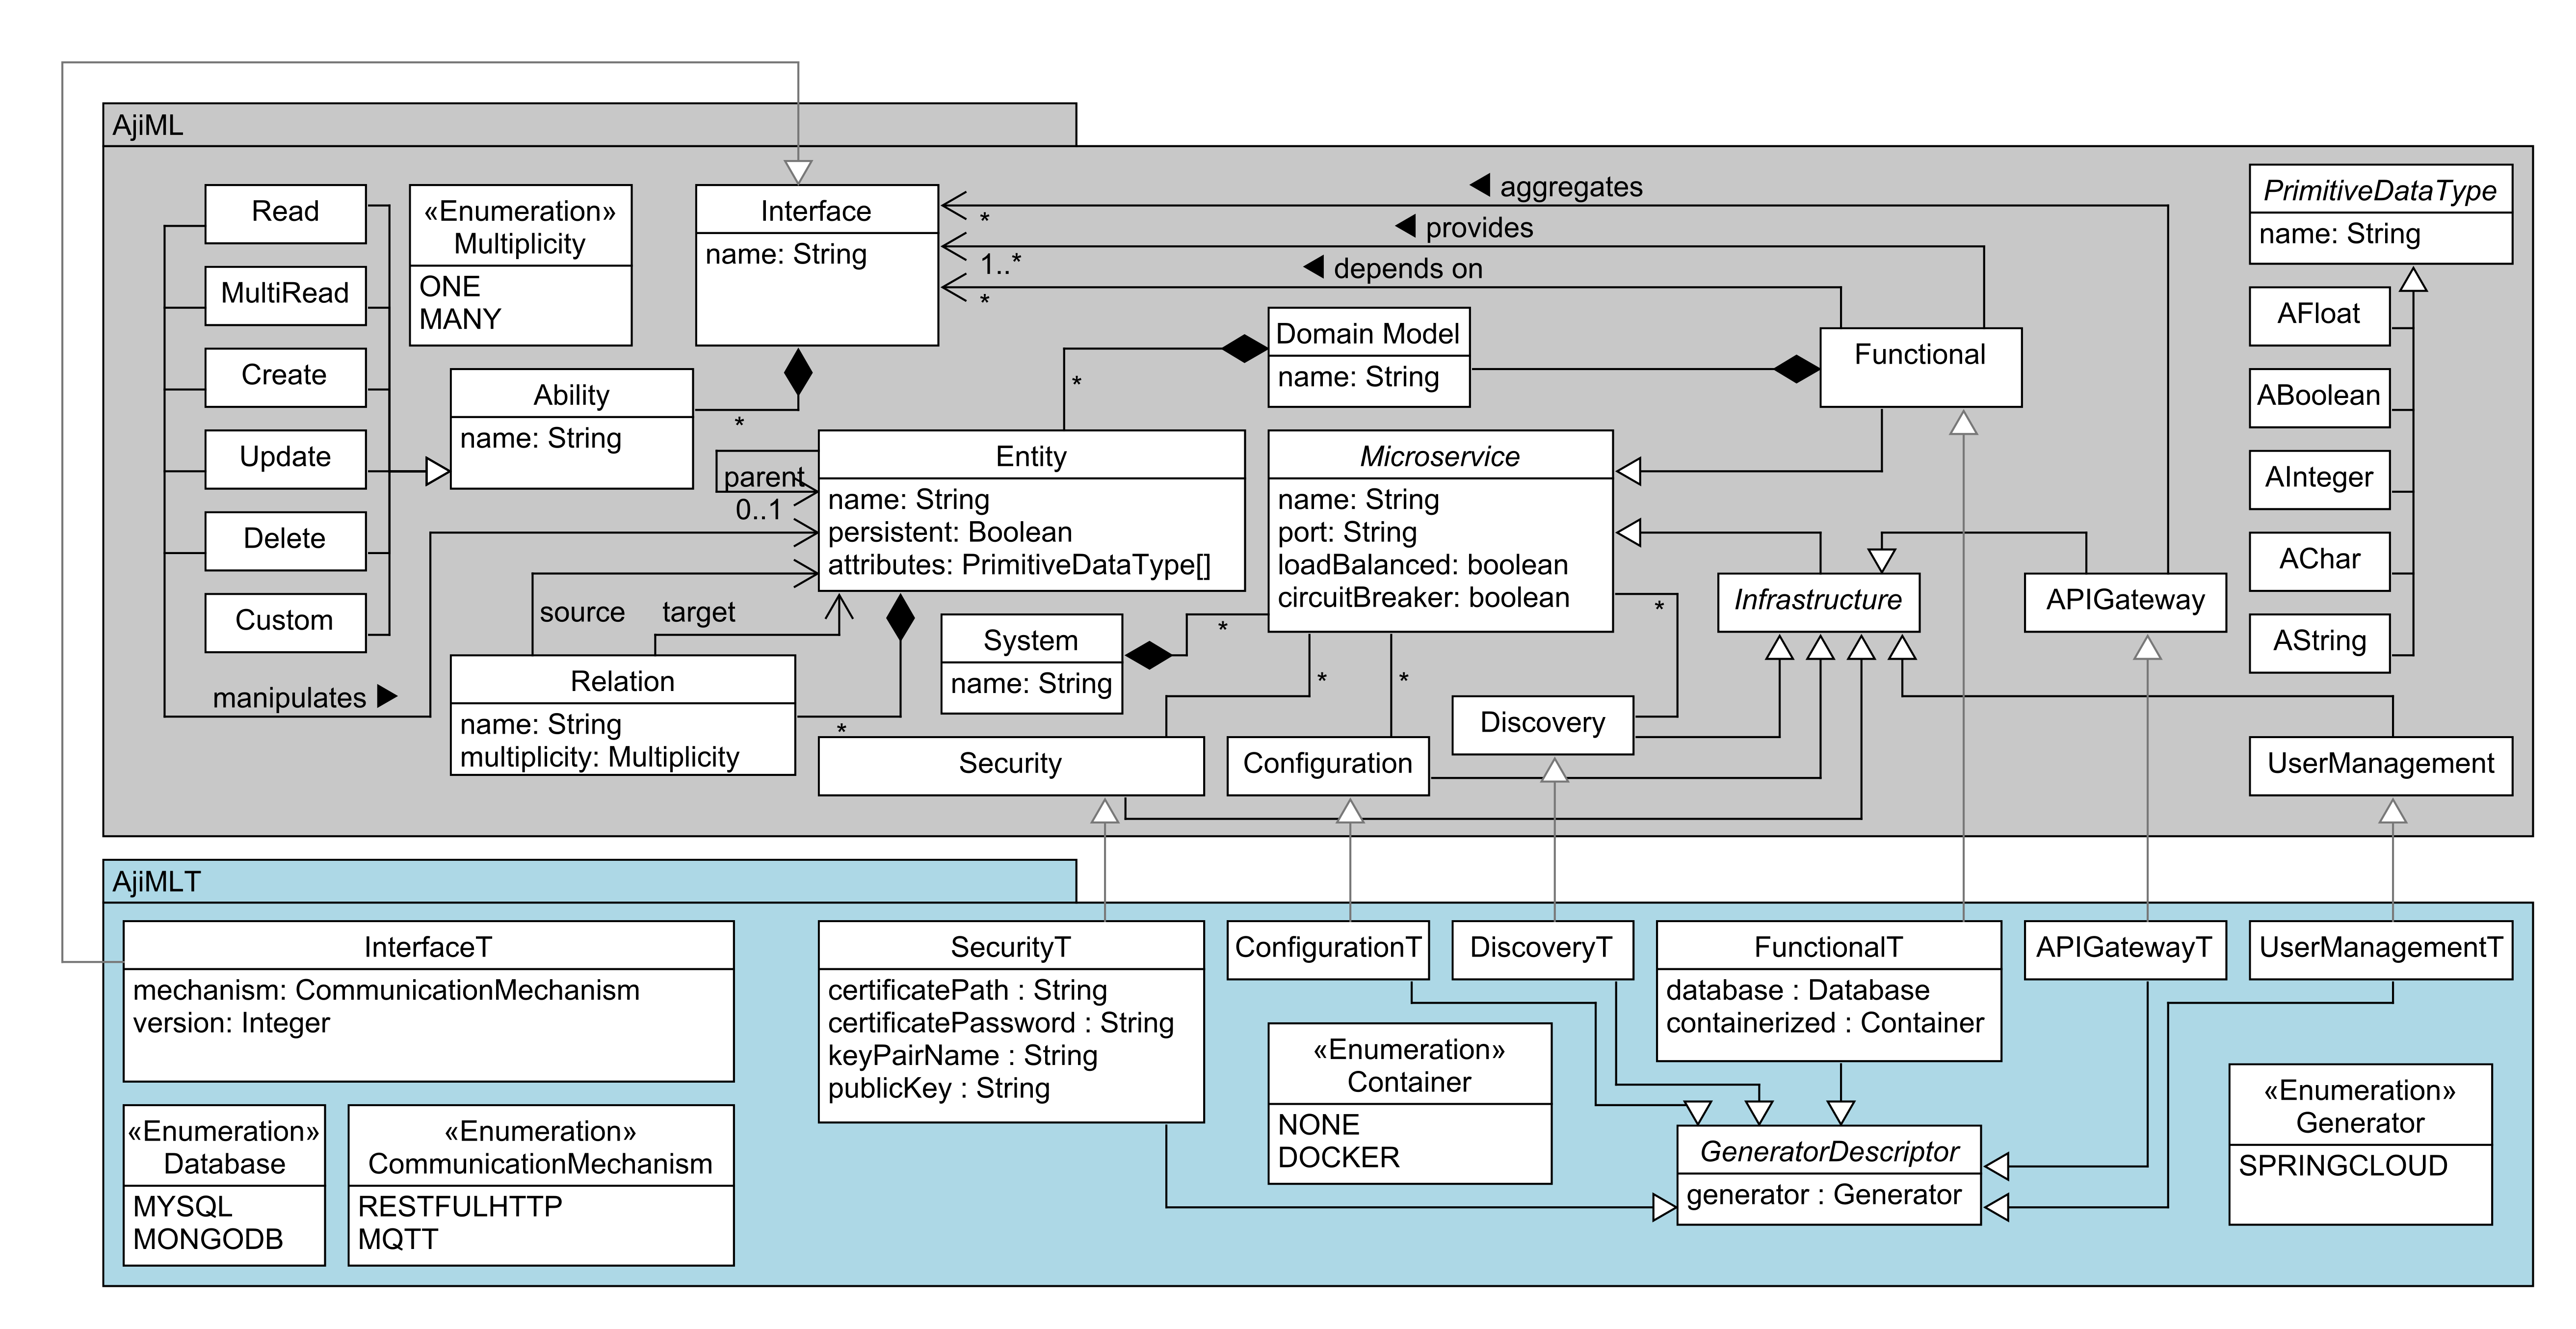
\includegraphics[width=\textwidth]{bilder/k3/k3_ajil.png}
\caption[Das AjiL Metamodell]{Das AjiL Metamodell \cite{ajilGithub}}
\end{figure}

AjiL bildet in seinem Metamodell verschiedene Aspekte von Microservice-Architekturen ab: So existieren Domain Models und Entities, welche Fachlichkeiten abbilden. Klassen wie Microservice, Security, Configuration oder Discovery bilden die technischen Metaklassen ab. Ebenso existieren Infrastruktur-Klassen wie Database oder Container. Das AjiMLT-Paket des Metamodells bildet konkrete Typen ab. So existiert beispielsweise ein Enum, welcher die Kommunikation einer Schnittstelle spezifiziert, konkret REST oder das Messaging-Protokoll MQTT.

Das AjiL-Metamodell bildet einen recht breiten Bereich der Microservice-Entwicklung ab, jedoch gibt es auch einige fehlende Abstraktionen, wie solche, die das Domain-Driven Design abbilden oder konkretere Cloud-Architekturen. AjiL setzt vieles davon implizit in den Generierungstemplates um, ohne explizite Modellklassen. Dadurch entsteht eine hohe Inflexibilität durch starre Teile des Templates.

Auch wenn AjiL einige interessante Ansätze bietet, auf denen man aufbauen kann, wie dessen Ansatz zum Schnittstellenmanagement und den ähnlichen Anforderungen an die zu generierenden Anwendungen, ist AjiL keine hinreichende Lösung, um DDD abzubilden und deploybare Anwendungen zu generieren.

\newpage

\subsubsection{Context Mapper}

\begin{figure}[ht]
\centering
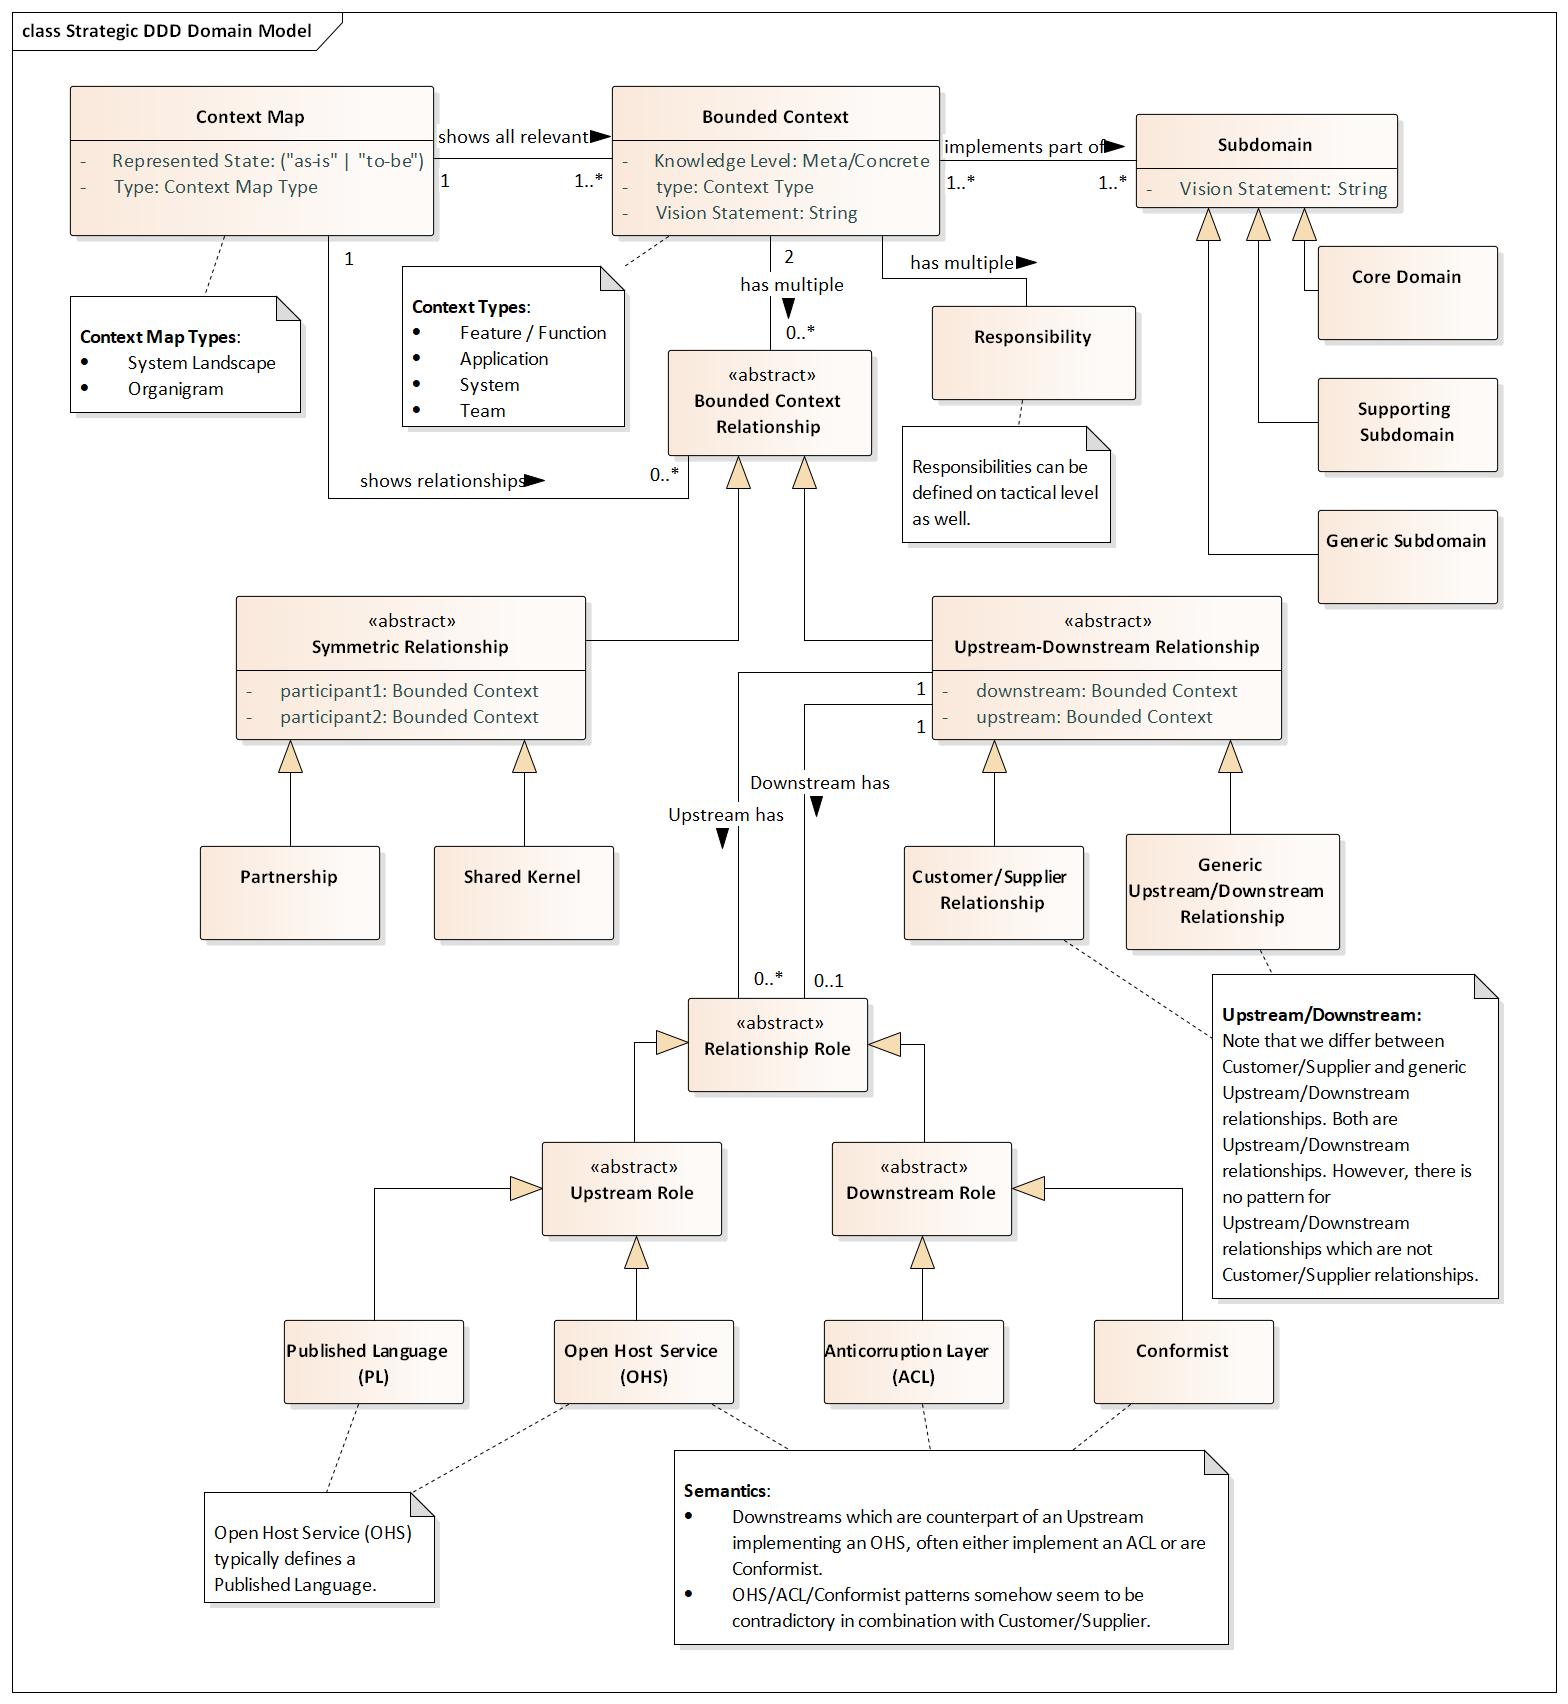
\includegraphics[height=15cm]{bilder/k3/k3_context_mapper.png}
\caption[Das Context Mapper Metamodell]{Das Context Mapper Metamodell \cite[S.3]{mapper}}
\end{figure}

Context Mapper definiert ein sehr umfassendes Metamodell, welches die Konzepte des DDD in höchster Ausführlichkeit modelliert. Context Mapper nutzt dieses, um Context Maps von Domänen zu generieren. Dementsprechend ist die Technologie keine Lösung, um Microservice-Anwendungen zu generieren. Jedoch ist die Modellierung eine umfassende Grundlage für eine Metamodellschicht, die das Strategic Design des DDD abbildet. Eine exakte Wiederverwendung bietet sich aus Gründen der Übersichtlichkeit nicht an, da Context Mapper so umfassend modelliert, dass eine auf generierende Anwendungen fokussierte Modellierung auch mit weniger Metamodell-Klassen auskommen kann. So ist beispielsweise die explizite Modellierung von Responsibilities oder Subdomains für zu generierende Microservices nicht notwendig. Aspekte der Visualisierung hingegen eignen sich sehr gut, um in einem dem Ziel dieser Arbeit angepassten Rahmen aufgegriffen zu werden.

\subsubsection{OCCI}

\begin{figure}[ht]
\centering
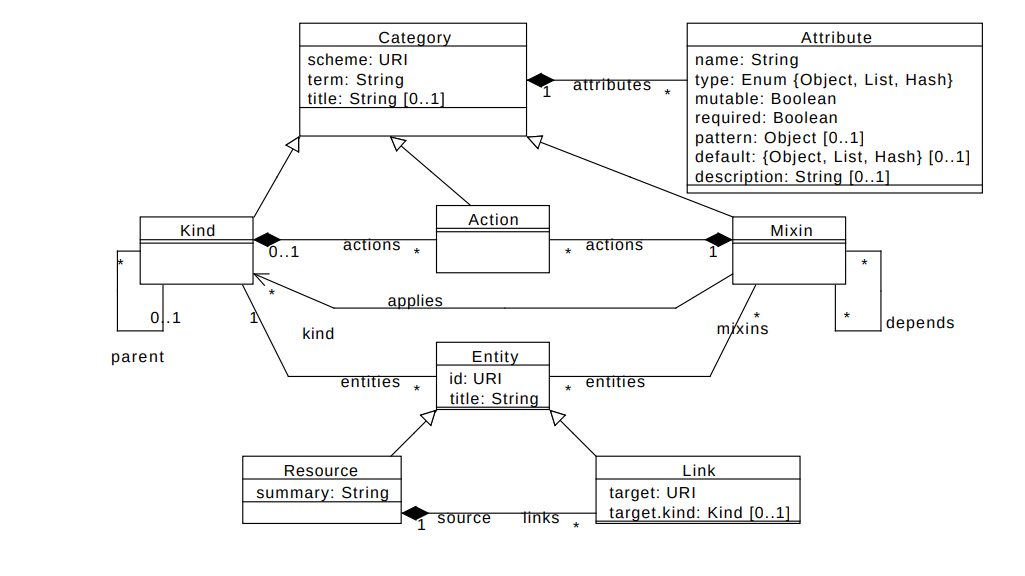
\includegraphics[width=\textwidth]{bilder/k3/k3_occi.png}
\caption[Das OCCI Metamodell]{Das OCCI Metamodell \cite[S.5]{edmonds}}
\end{figure}

Das Metamodell des Open Cloud Computing Interface (OCCI) stellt eine kompakte Abstraktion dar, um Cloud-Ressourcen und -Dienste effektiv zu modellieren. Es vermeidet eine direkte Abstraktion von spezifischen Konzepten wie Container oder Deployments. Stattdessen verwendet OCCI allgemeinere Klassen wie Entity, Resource und Link, um eine breite Palette von Cloud-Konzepten und Beziehungen darzustellen.

Beispielsweise kann eine Entity in diesem Modell einen konkreten Cloud-Service oder eine virtuelle Maschine repräsentieren, während Resource für spezifische Dienste wie Speicherplatz oder Rechenkapazitäten steht. Link kann genutzt werden, um die Verbindungen zwischen verschiedenen Ressourcen oder Diensten abzubilden, wie etwa die Zuordnung eines Netzwerkdienstes zu einem bestimmten Container. Dieser abstrakte Ansatz ermöglicht es, das Modell flexibel und anpassbar für eine Vielzahl von spezifischen Cloud-Umgebungen und Anwendungsfällen zu gestalten.

Trotz der Fähigkeit der Technologie, Cloud-Infrastrukturen umfassend zu modellieren und zu generieren, ist sie für die Anforderungen dieser Arbeit aufgrund ihrer komplexen Handhabung und der Fokussierung auf Infrastruktur anstatt auf Anwendungssoftware weniger geeignet. 

\begin{figure}[ht]
\centering
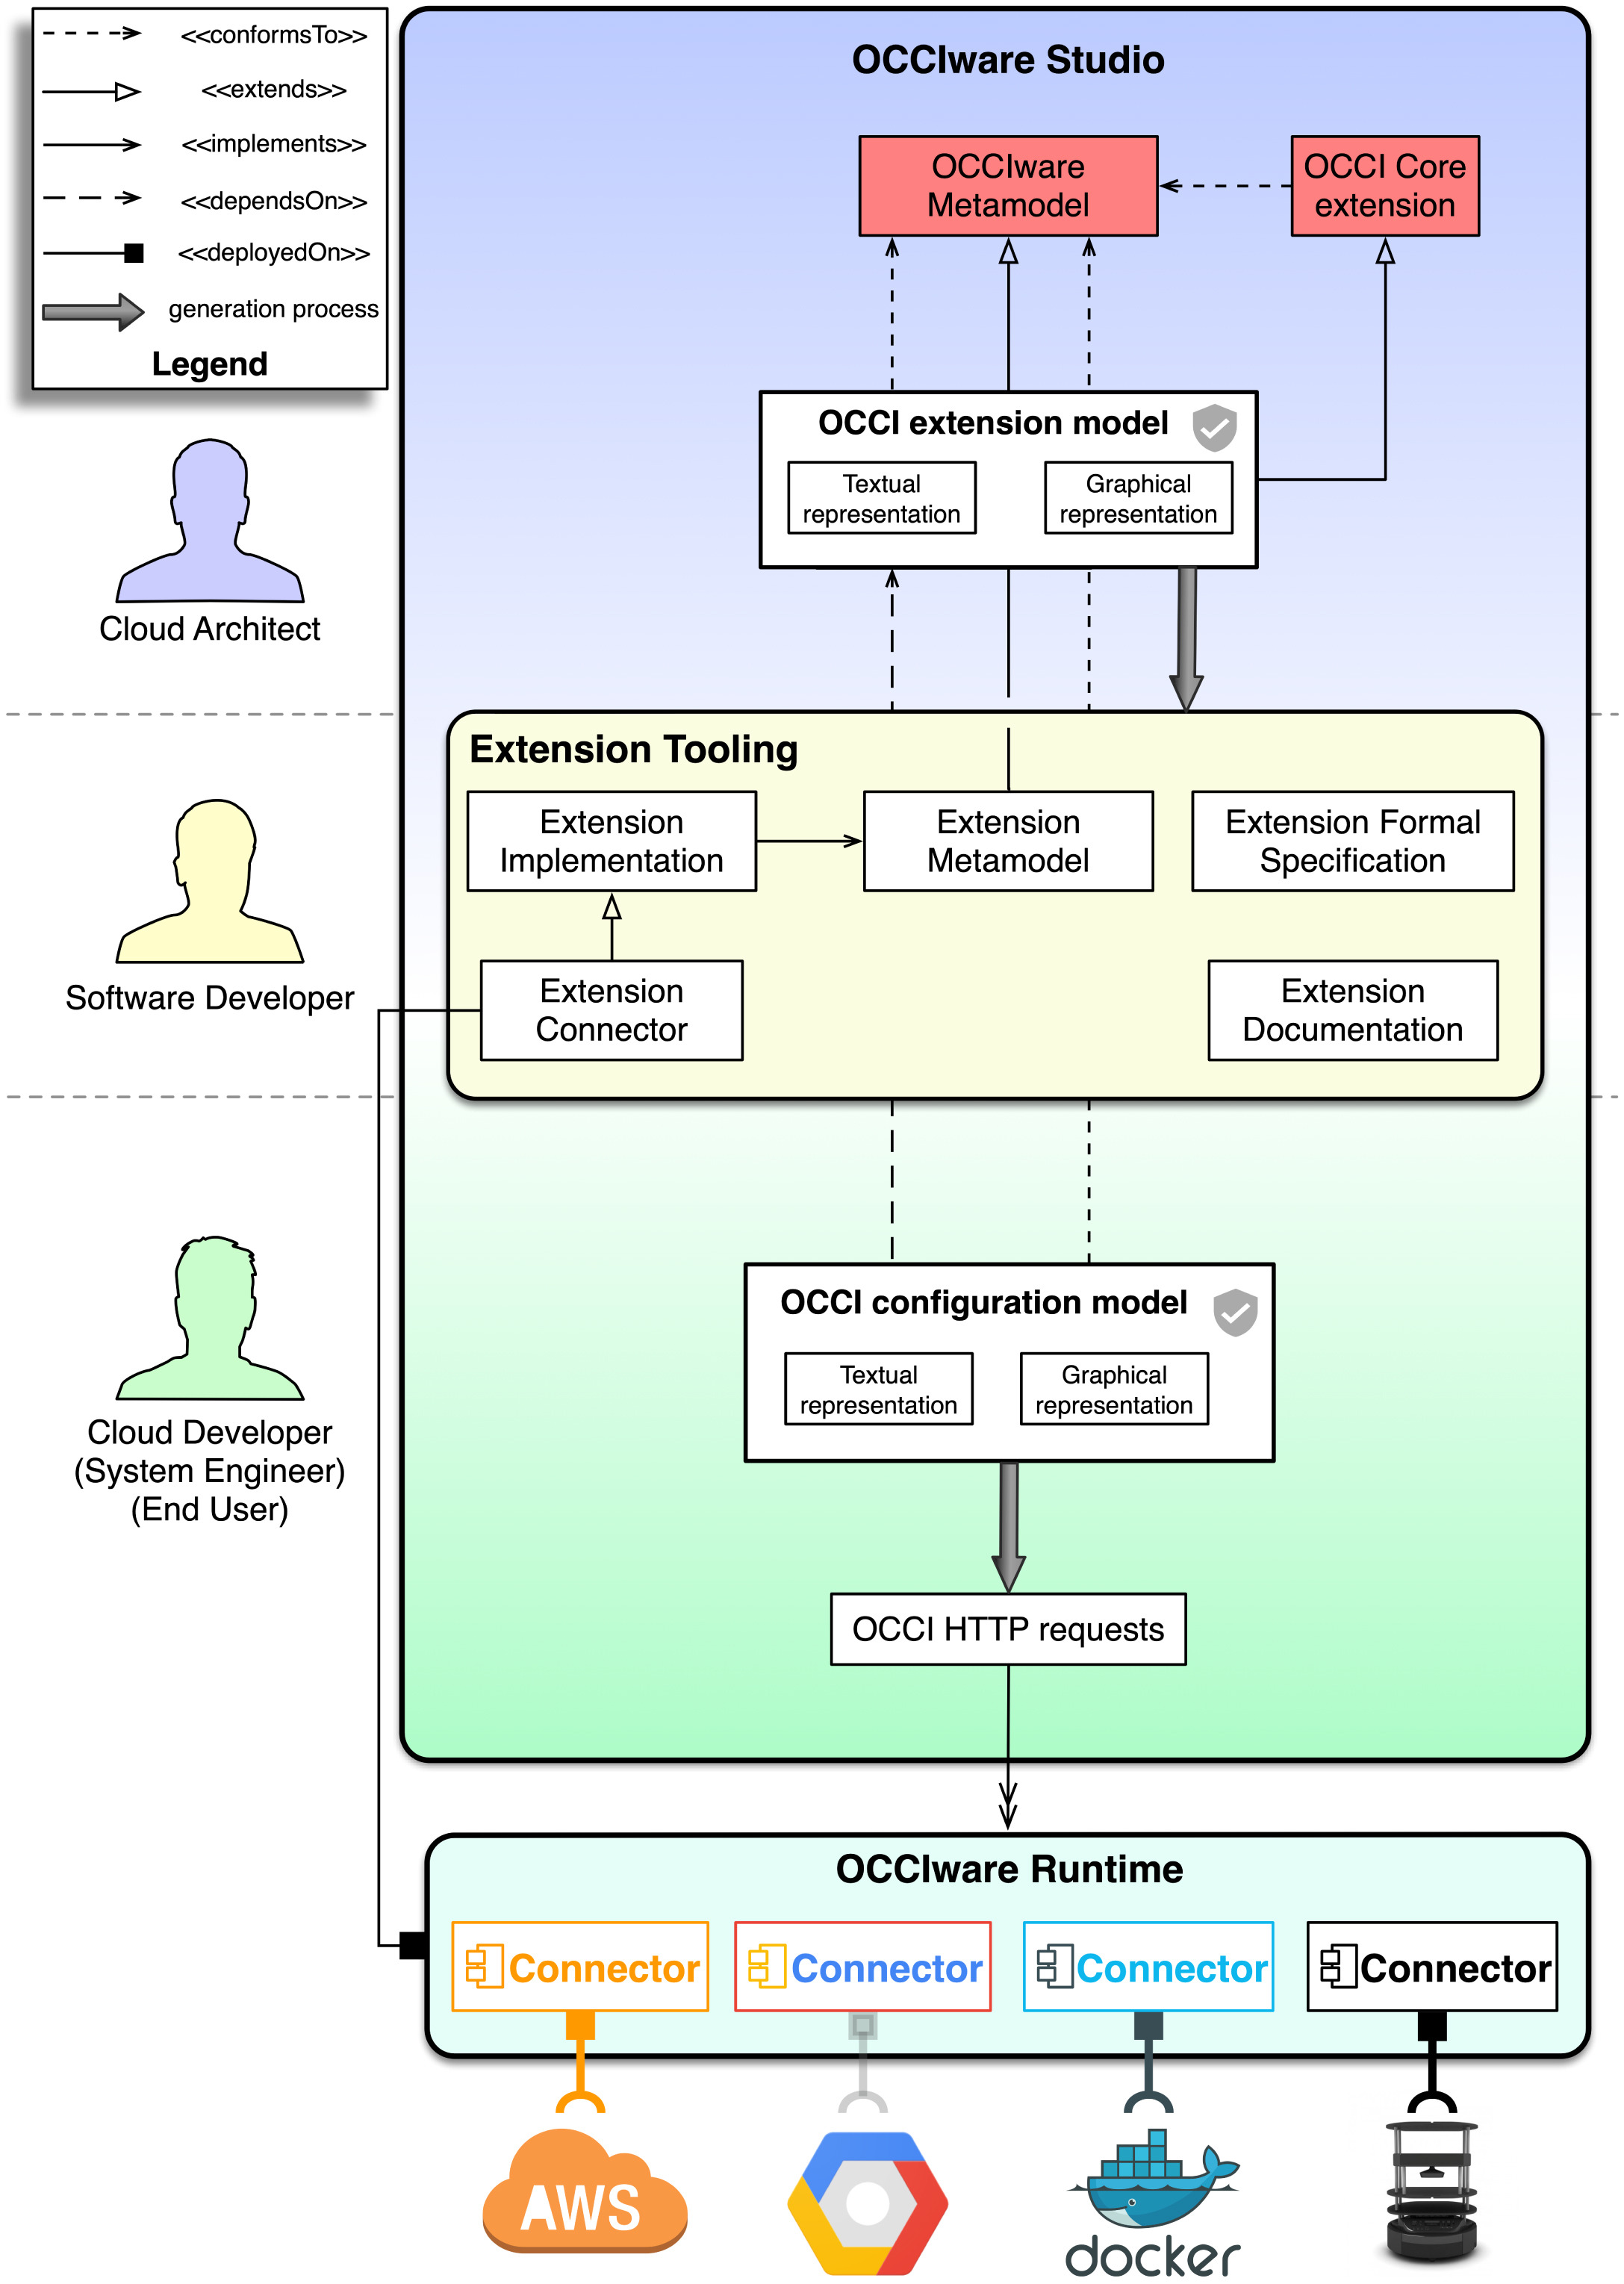
\includegraphics[height=12cm]{bilder/k3/k3_occi_2.jpg}
\caption[OCCIware Anwendungsumgebung]{Das OCCI Metamodell als Teil der komplexen OCCIware Anwendungsumgebung \cite{zalila}}
\end{figure}

\newpage


\subsubsection{ARGON}

Die Technologie ARGON strukturiert den Ansatz, Cloud-Infrastrukturen modellbasiert zu entwickeln, in mehrere Ebenen. Im Gegensatz zu OCCI, das ein umfangreiches Anwendungsframework bietet, konzentriert sich ARGON auf die Definition eines plattformunabhängigen Metamodells (PIM) sowie spezifischer Metamodelle (PSM) für AWS und Microsoft Azure. Mittels M2M-Transformationen ist eine gegenseitige Umwandlung möglich. Zudem sind M2T-Transformationen vorgesehen, um Infrastructure-as-Code mittels Ansible oder Terraform zu erzeugen.

In diesem Kontext erweist sich ARGON als deutlich geeigneter als OCCI, da es sich auf die praxisnahe Erstellung von Software-Komponenten konzentriert, die durch ein konkreteres Metamodell definiert werden, anstatt auf einen abstrakten, plattformübergreifenden Cloud-Baukasten. Auch der hierarchische Ansatz und das in Relation setzen von Cloud-spezifischen Modellen sind sinnvoll aufgreifbare Konzepte.
Die Problematik der fehlenden Anwendungsebene liegt jedoch weiterhin vor. Die Entwicklung einer Schnittstelle zu ARGON wäre eine Möglichkeit, diese zu lösen.

Stattdessen soll im Rahmen dieser Arbeit, gemäß dem Fokus auf das lauffähige Deployment von Microservice-Architekturen, eine Lösung entwickelt werden, die Anwendungsmodellierung und Deployment für eine konkrete Zielplattform in einem Metamodell vereint. Dabei kann der ARGON-Ansatz plattformunabhängige Modellelementen und spezifischer Modellelemente zu modellieren integriert werden. 

\begin{figure}[ht]
\centering
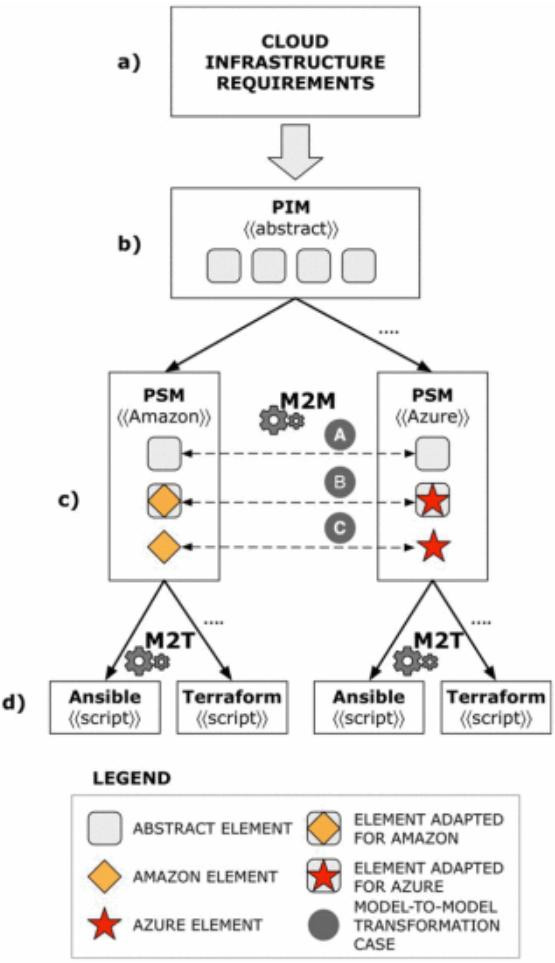
\includegraphics[height=11cm]{bilder/k3/k3_argon.jpg}
\caption[Architekturkonzept von ARGON]{Architekturkonzept von ARGON \cite{argon}}
\end{figure}

\subsection{Auswahl der Technologie}

Die Umsetzung des Metamodells erfolgt mit dem Eclipse Modeling Framework (Abk.: EMF), einem quelloffenen Java-Framework. Weiterhin kommen die ebenfalls quelloffenen Frameworks Eclipse Sirius, das die Visualisierung von Modellen ermöglicht, und Acceleo, das aus EMF-Modellen Code generieren kann, zum Einsatz. Diese stehen Eclipse als Plugins zur Verfügung. Die generierten Anwendungen sollen die Programmiersprache Java verwenden. Zudem wird das Spring Framework eingesetzt, welches die Implementierung verschiedenster Strukturen vereinfacht. Als Technologie zur Umsetzung von eventgetriebener Architektur wird Apache Kafka verwendet. Die generierten Applikationen sollen mittels Gradle gebaut und als Docker Image ausgeführt werden können. Als Cloud-Infrastruktur wird die Google Cloud gewählt, in welcher die Anwendungen auf einem Kubernetes-Cluster laufen sollen. Mit der Unix-Shell Bash werden dazu nötige Skripte umgesetzt. Als Datenbank Technologie wird die in-memory Datenbank H2 verwendet.


%%%%%%%%%%%%%%%%%%%%%%%%%%%%%%%%%%%%%%%%%%%%%%%%%%%%%%%%%%%%%%%%%%%%%%%%%%%%%%%%%%%%%%%%%%%%%%%%%%%%%%%%%%%%%%%%%%%%
%			DSL
%%%%%%%%%%%%%%%%%%%%%%%%%%%%%%%%%%%%%%%%%%%%%%%%%%%%%%%%%%%%%%%%%%%%%%%%%%%%%%%%%%%%%%%%%%%%%%%%%%%%%%%%%%%%%%%%%%%%

\newpage
\section{Entwicklung der eigenen DSL}

\subsubsection{Grundkonzept - Definition verschiedener Modellschichten}

Um ein Metamodell für Microservice-Architekturen zu konzipieren, wird zunächst ein plausibles, konkretes Modell betrachtet. Basierend auf einer Analyse dieses Modells soll beginnend ein grundlegender Ansatz gewählt werden, der im Kontext einer Abstraktion sinnvoll erscheint.

Hierzu wird ein Beispielmodell (Abbildung 4.6) eingeführt, das eine Domäne umfasst. Diese besteht aus den Kontexten Customer und Marketing, die eine Customer/Supplier-Beziehung haben. Weiterhin gibt es Microservices zu diesen Kontexten, die über eine Schnittstelle miteinander kommunizieren. Die Ausführungsumgebung wird mit spezifischer Servicekonfiguration und einem Modellelement, das die Cloud-Umgebung beschreibt – hier die Google Cloud-Infrastruktur – ebenfalls modelliert.

Bei der Betrachtung wird folgendes festgestellt: Die existierenden Modellelemente lassen sich in fachliche Elemente, technische Elemente oder Infrastrukturelemente gruppieren. Diese Gruppierung wird als gemeinsame Schicht definiert. Innerhalb ihrer Schicht haben die Elemente Beziehungen zu anderen Modellelementen derselben Schicht. Weiterhin können Beziehungen existieren, die über diese Schichten hinausgehen, das heißt, es gibt Abbildungen von Elementen einer Schicht auf Elemente anderer Schichten.

Da durch Schichten die mögliche Komplexität besser gegliedert und somit einfacher handhabbar gemacht wird, wird das Metamodell ebenfalls schichtbasiert konzipiert. Neben der Zuordnung der Konzepte in die passende Schicht muss dabei erforscht werden, wie die Beziehungen innerhalb und zwischen den Schichten umgesetzt werden können. Nach abschließender Betrachtung aller Schichten muss das Metamodell im Kontext der Konzeption von Codegenerierung und Migrationsfähigkeiten weiterhin iterativ überprüft und gegebenenfalls nachgebessert werden. Hierbei werden die Bewertungskriterien aus den einleitenden Überlegungen berücksichtigt.

\begin{figure}[ht]
\centering
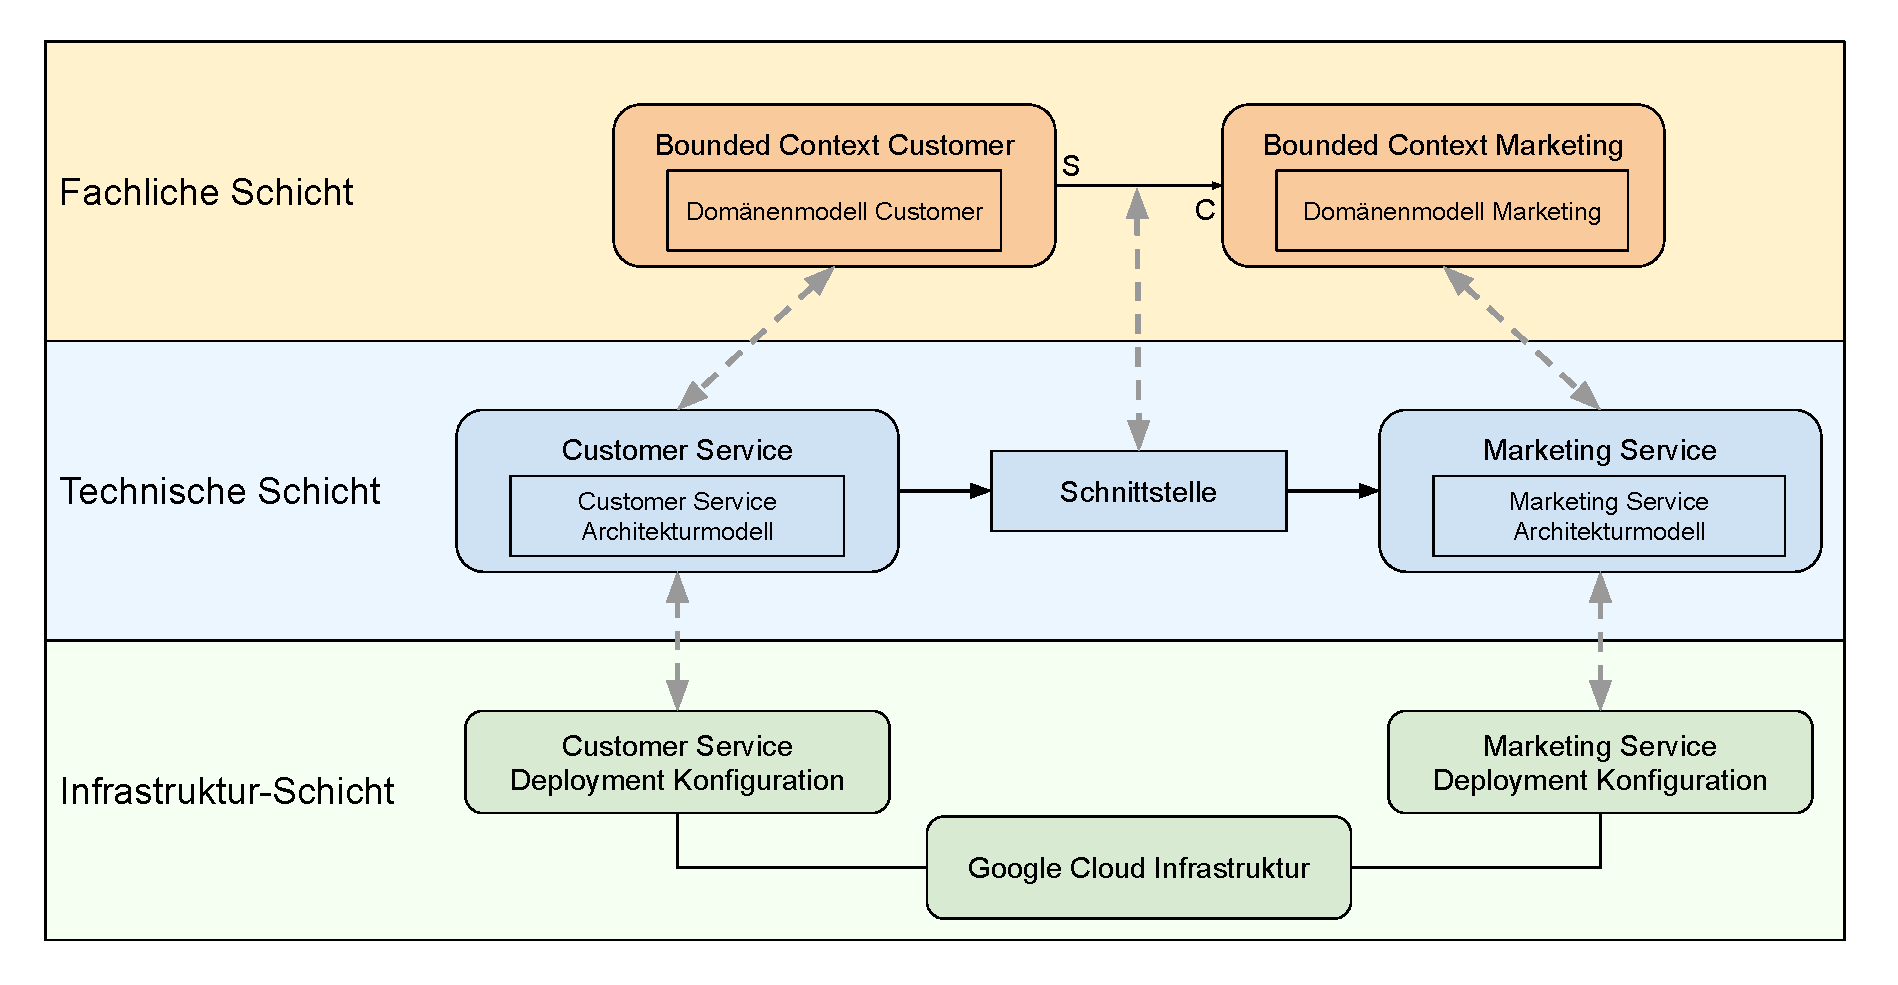
\includegraphics[width=0.8\textwidth]{bilder/k3/konzept.pdf}
\caption[Erkennbare Schichten in einem Modell einer Microservice-Architektur]{Erkennbare Schichten in einem Modell einer Microservice-Architektur}
\end{figure}

%%%%%%%%%%%%%%%%%%%%%%%%%%%%%%%%%%%%%%%%%%%%%%%%%%%%%%%%%%%%%%%%%%%%%%%%%%%%%%%%%%%%%%%%%%%%%%%%%%%%%%%%%%%%%%%%%%%%
%			Fachl. MDD
%%%%%%%%%%%%%%%%%%%%%%%%%%%%%%%%%%%%%%%%%%%%%%%%%%%%%%%%%%%%%%%%%%%%%%%%%%%%%%%%%%%%%%%%%%%%%%%%%%%%%%%%%%%%%%%%%%%%

\subsection{Modellierung des Model-Driven Designs}

Beginnend wird das DDD in das Metamodell integriert. Dieses findet sich in einer Klasse für die fachlichen Schicht, der \glqq DomainModelLayer\grqq{}, wieder. Die Schicht besteht aus drei Abstraktionsebenen: dem Domänenmodell, dem MDD und dem Strategic Design. Im Folgenden werden diese farblich unterschieden und die detailliertere Konzeption ausgeführt. Zur besseren Übersicht werden dabei bereits eingeführte Klassen und Relationen nach Möglichkeit ausgeblendet.

\begin{figure}[ht]
\centering
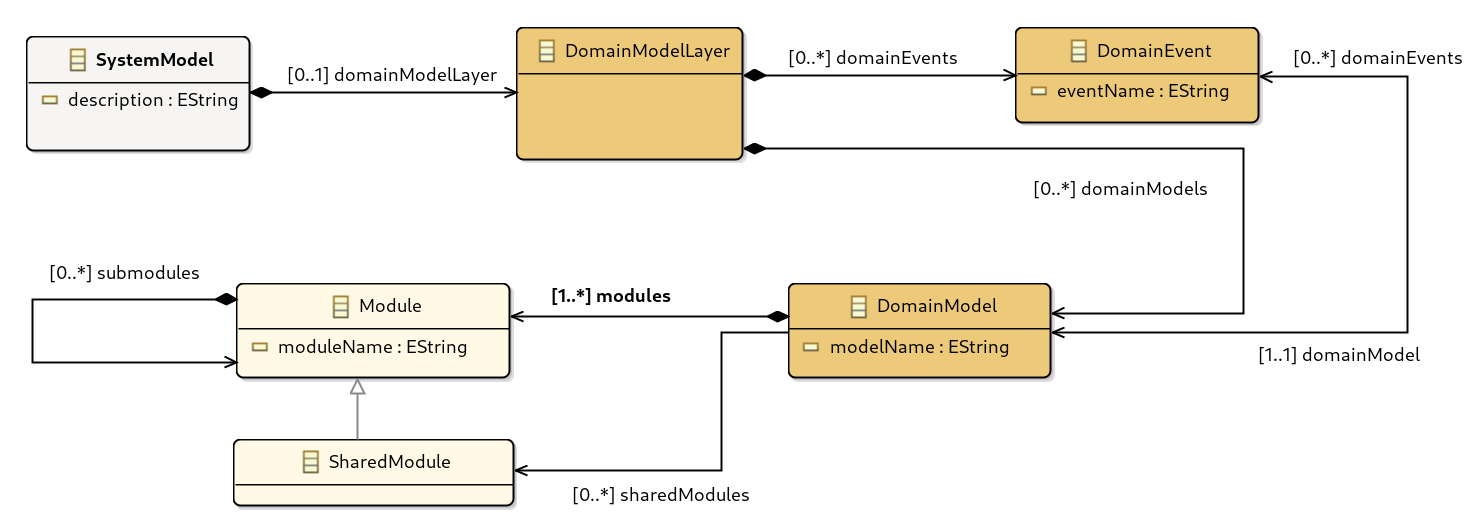
\includegraphics[width=\textwidth]{bilder/k4/1.png}
\caption[Metamodell - Fokus: Fachliche Schicht, Domänenmodelle und Pakete]{Metamodell - Fokus: Fachliche Schicht, Domänenmodelle und Pakete}
\end{figure}

Die fachliche Schicht besteht aus beliebig vielen benannten \glqq DomainModels\grqq{}. Weiterhin enthält diese ebenfalls beliebig viele \glqq DomainEvents\grqq{}. Durch eine bidirektionale Assoziation kann die Referenz von einem DomainModel zu verschiedenen Events beschrieben werden. Die Events selbst sind dabei nur einem DomainModel zugeordnet. Ein hypothetisches Event, das in mehreren Domänenmodellen vorkommt, wäre in dem Analyseprozess einer Problemdomäne ein Indiz für ein nicht erkanntes Domänenmodell.

Das DomainModel besitzt weiterhin Module, umgesetzt mit einer Klasse \glqq Module\grqq{}, welche wiederum Submodule enthalten können. Es zeigte sich während der Konzeption, dass es vorteilhaft ist, dass jedes DomainModel mindestens ein Modul besitzen muss. Diese Entscheidung erleichtert einerseits eine strukturiertere Codegenerierung. Andererseits wird dadurch eine deutlich einfachere Besitzbeziehung für das noch einzuführende \glqq ModelElement\grqq{} realisiert. Auch der Aufwand für die  Konzeption der dazugehörigen konkreten Syntax sinkt bedeutend. Die von Module abgeleitete Klasse \glqq SharedModule\grqq{} beschreibt Module, die in mehreren DomainModels vorkommen können. Diese Modellierung ist notwendig, um eine korrekte Umsetzung des noch einzuführenden Konzepts Shared Kernel zu ermöglichen.

\newpage

\begin{figure}[ht]
\centering
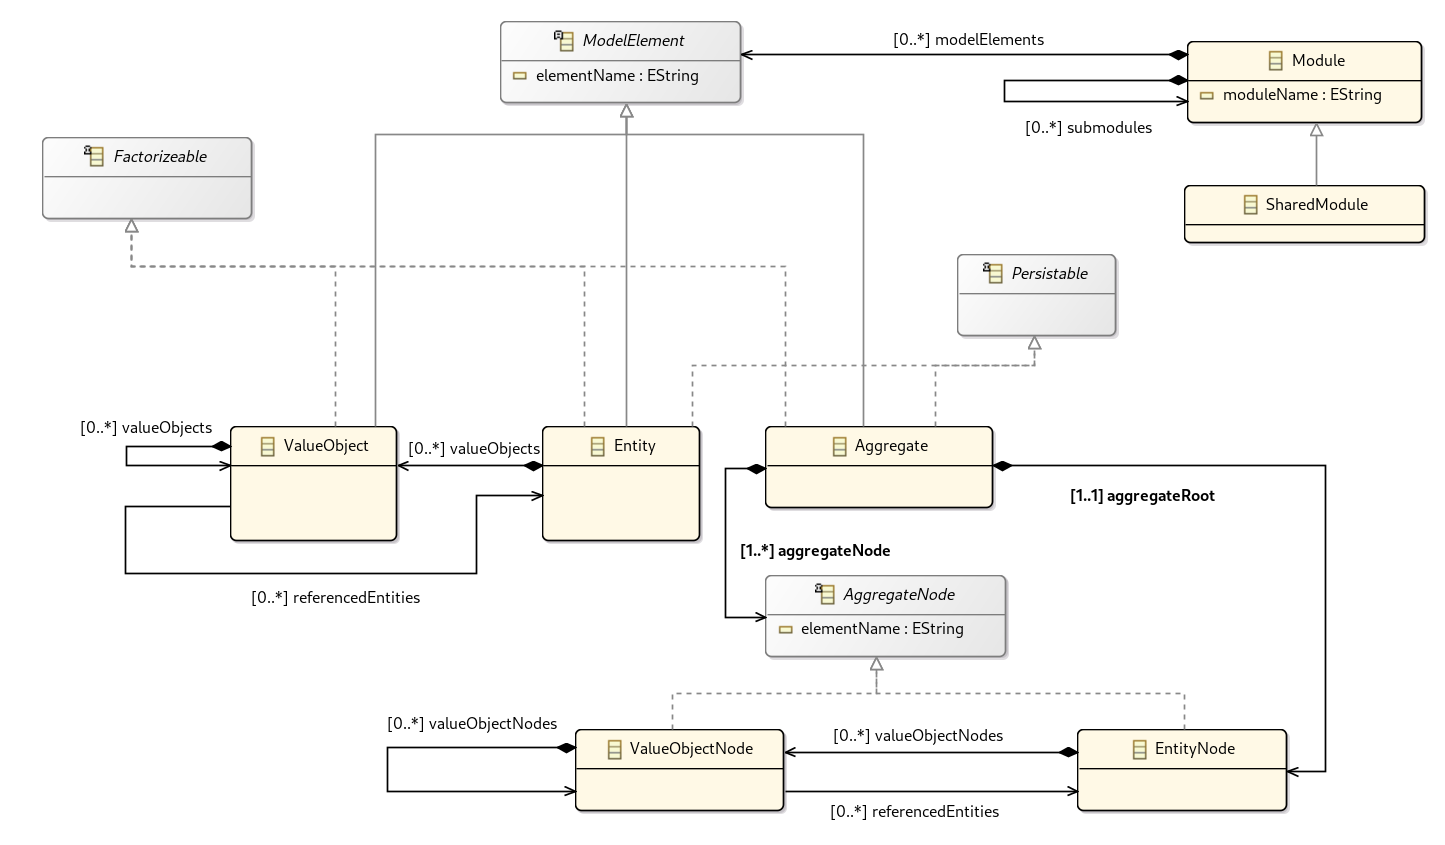
\includegraphics[width=\textwidth]{bilder/k4/2.png}
\caption{Metamodell - Fokus: Entitiy, Value Object und Aggregate}
\end{figure}

Als abstrakte Basisklasse des MDD wird das ModelElement entworfen, welches in Module beliebig oft enthalten sein kann. Davon lassen sich die aus dem MDD bekannten Konzepte der Entities, Value Objects und Aggregates als Klassen ableiten. Nach dem DDD sind diese von Factories erzeugbare Objekte, umgesetzt durch die Einführung einer Schnittstelle namens \glqq Factorizable\grqq{}. Dies wurde symmetrisch für Entities und Aggregates mit der Schnittstelle \glqq Persistable\grqq{} umgesetzt. Die Besitz- und Referenzrelation für Value Objects und Entities ist ebenso eine direkte Umsetzung der Definition des DDD.

Die modellgetreue Definition des Aggregates gestaltet sich schwierig. Die Umsetzung einer von außen zugreifbaren Entity-Wurzel mit von außen nicht zugreifbaren Blättern, welche Entities oder Value Objects sind, mit denselben Relationen, die aber nur untereinander gelten, hat sich als nicht elegant umsetzbar erwiesen. Der Versuch, eine einzige Entity-Klasse im Modell abzubilden, führte dazu, dass Elemente, die eigentlich vom Aggregate abgekapselt sein sollten, Zugriff darauf erhalten könnten. Diese Kapselung von Beziehungen muss durch eigene Klassen für Entities und Value Objects in einem Aggregate realisiert werden. Dementsprechend wird eine Klasse \glqq EntityNode\grqq{}, die einmalig als Wurzel existieren muss, modeliert. Weiterhin wird dazu eine abstrakte Klasse \glqq AggregateNode\grqq{}, und die diese ableitenden Klassen \glqq EntityNode\grqq{} und \glqq ValueObjectNode\grqq{} eingeführt.

\newpage


\begin{figure}[ht]
\centering
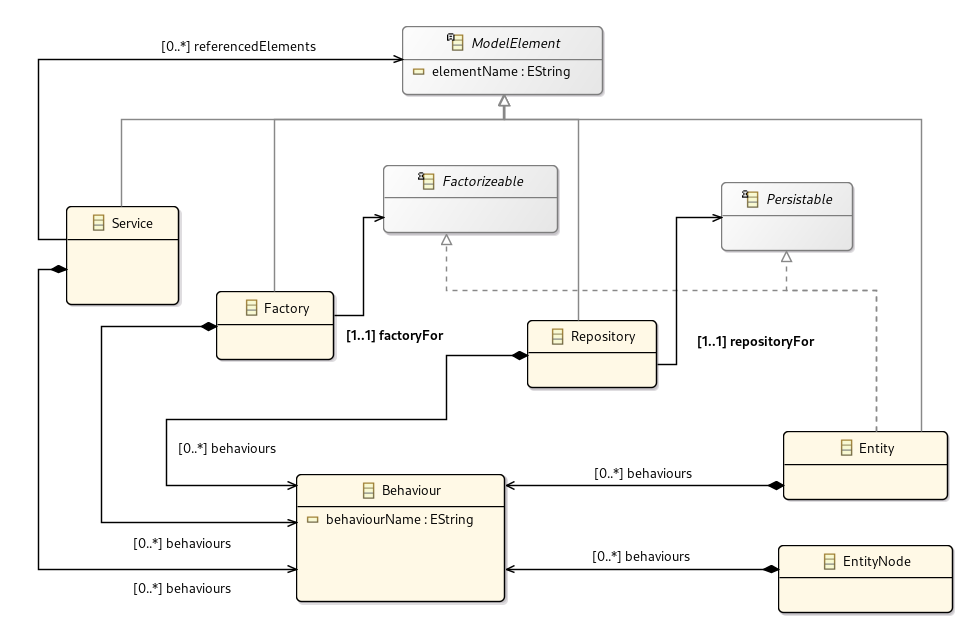
\includegraphics[width=\textwidth]{bilder/k4/3.png}
\caption{Metamodell - Fokus: Service, Repository, Factory und Behaviour}
\end{figure}

Es werden zu den MDD-Konzepten passenden Klassen \glqq Service\grqq{}, \glqq Factory\grqq{} und \glqq Repository\grqq{}, welche ebenfalls Ableitungen von ModelElement sind, konzipiert. Die bereits eingeführten Schnittstellen Factorizeable und Persistable werden von Factory und Repository passend referenziert. Dabei sind sowohl Factory als auch Repository je Objekt ihrer Klasse nur maximal einem, die Schnittstelle implementierenden, Objekt zugewiesen. Die Klasse Service hat weiterhin eine Assoziation zu beliebig vielen ModelElements, mit dem Zweck, Anwendungslogik umsetzen zu können. Eine Klasse Behaviour wird weiterhin zusätzlich eingeführt. Dies zeigte sich als notwendig, um das Verhalten in der Generierung und Modellierung präzise beschreiben zu können.


%%%%%%%%%%%%%%%%%%%%%%%%%%%%%%%%%%%%%%%%%%%%%%%%%%%%%%%%%%%%%%%%%%%%%%%%%%%%%%%%%%%%%%%%%%%%%%%%%%%%%%%%%%%%%%%%%%%%
%			Fachl. Strategic Design
%%%%%%%%%%%%%%%%%%%%%%%%%%%%%%%%%%%%%%%%%%%%%%%%%%%%%%%%%%%%%%%%%%%%%%%%%%%%%%%%%%%%%%%%%%%%%%%%%%%%%%%%%%%%%%%%%%%%
\newpage
\subsection{Modellierung des Strategic Designs}

\begin{figure}[ht]
\centering
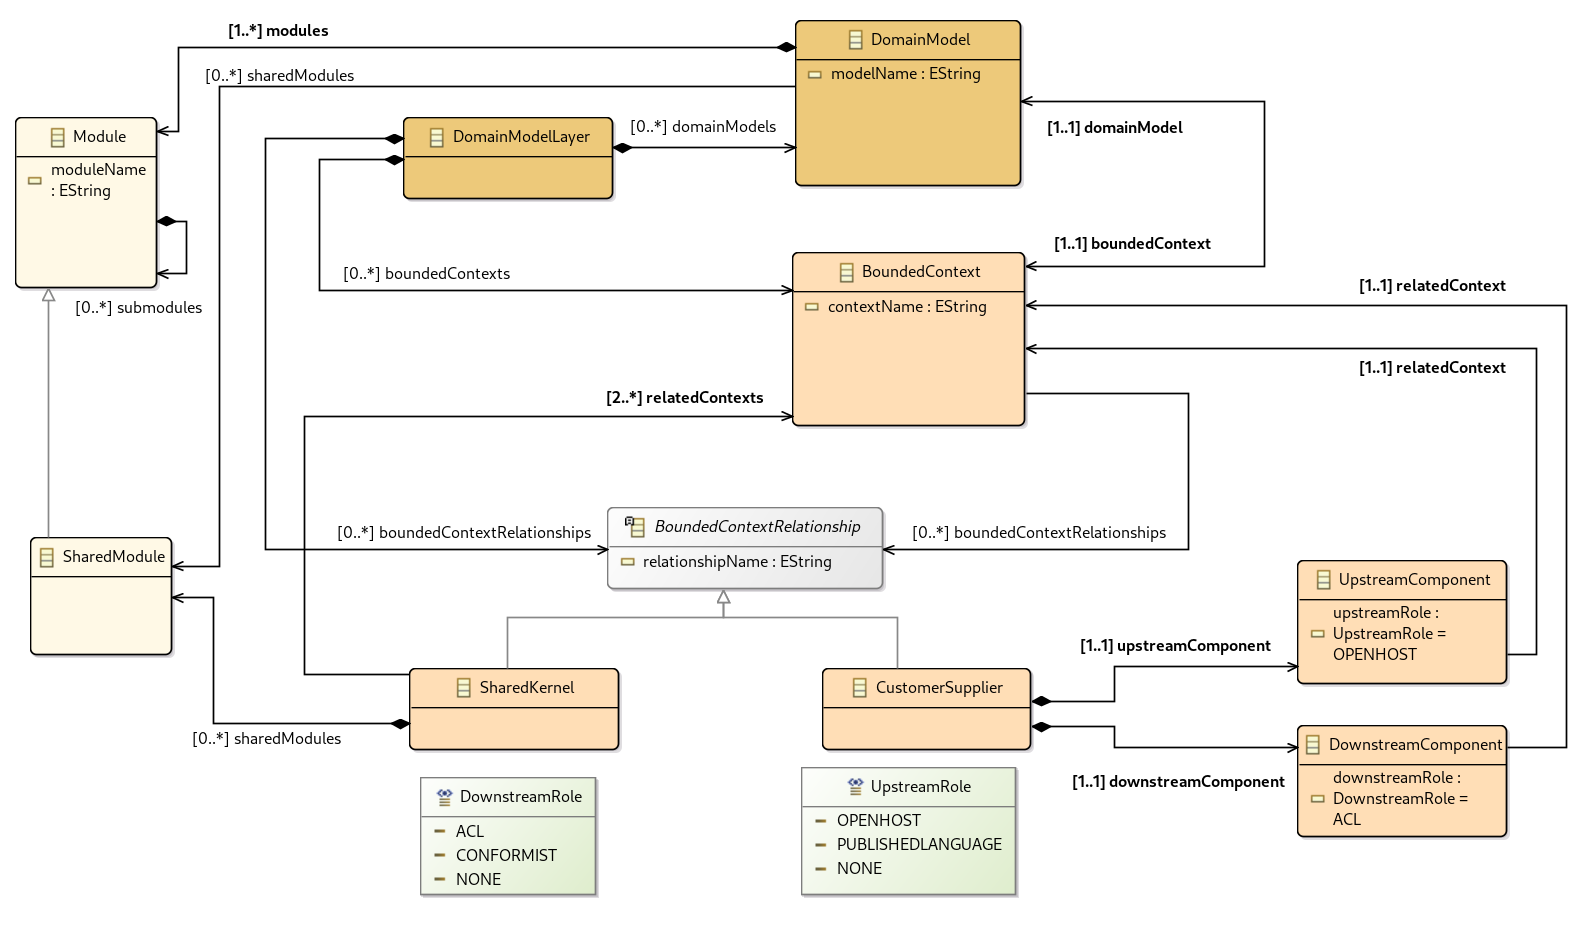
\includegraphics[width=\textwidth]{bilder/k4/4.png}
\caption{Metamodell - Fokus: Strategic Design}
\end{figure}

Die Modellierung des Bounded Context im Metamodell beginnt mit der Zuweisung der zugehörigen Klasse \glqq BoundedContext\grqq{} als Teil des DomainModelLayer. Weiterhin wird nach dem DDD eine Ist-Beziehung zwischen DomainModel und BoundedContext eingeführt. In Betrachtung des Strategic Design soll der Bounded Context explizit vom DomainModel unterscheidbar sein, da im Folgenden die Beziehungen dieser untereinander im Vordergrund stehen, während das DomainModel den Blick in den Bounded Context symbolisiert. Ebenso Teil des DomainModelLayer ist die abstrakte Klasse \glqq BoundedContextRelationship\grqq, welche beliebig oft von einem Bounded Context referenziert werden kann. Diese beschreibt Beziehungen als eigene Objekte, analog zu dem Konzept von ContextMapper. \glqq SharedKernel\grqq{} und \glqq CustomerSupplier\grqq{} sind die zwei davon abgeleiteten Klassen. CustomerSupplier besitzt weiterhin jeweils eine sendende und empfangende Komponente, welche auf genau einen Bounded Context verweist. Im Gegensatz zu ContextMapper reicht hier eine reduzierte Modellierung der Konzepte des Strategic Design. Dies zeigte sich bei der Konzeption von Visualisierung und Generierung. Dabei ergab sich, dass die Modellierung der übrigen Strategic Design Konzepte als statische Enumerationen hinreichend ist. SharedKernel enthält außerdem noch die bereits erwähnte Referenz auf das SharedModule. Dies ist notwendig, um bei der Beschreibung des DomainModels dieses korrekt zu referenzieren. Das Fehlen kann somit zu einer unvollständigen Beschreibung führen, wodurch möglicherweise wichtige Aspekte zum Verständnis des Modells fehlen würden.


%%%%%%%%%%%%%%%%%%%%%%%%%%%%%%%%%%%%%%%%%%%%%%%%%%%%%%%%%%%%%%%%%%%%%%%%%%%%%%%%%%%%%%%%%%%%%%%%%%%%%%%%%%%%%%%%%%%%
%			Techn
%%%%%%%%%%%%%%%%%%%%%%%%%%%%%%%%%%%%%%%%%%%%%%%%%%%%%%%%%%%%%%%%%%%%%%%%%%%%%%%%%%%%%%%%%%%%%%%%%%%%%%%%%%%%%%%%%%%%

\newpage
\subsection{Modellierung der technischen Modellebene}

\begin{figure}[ht]
\centering
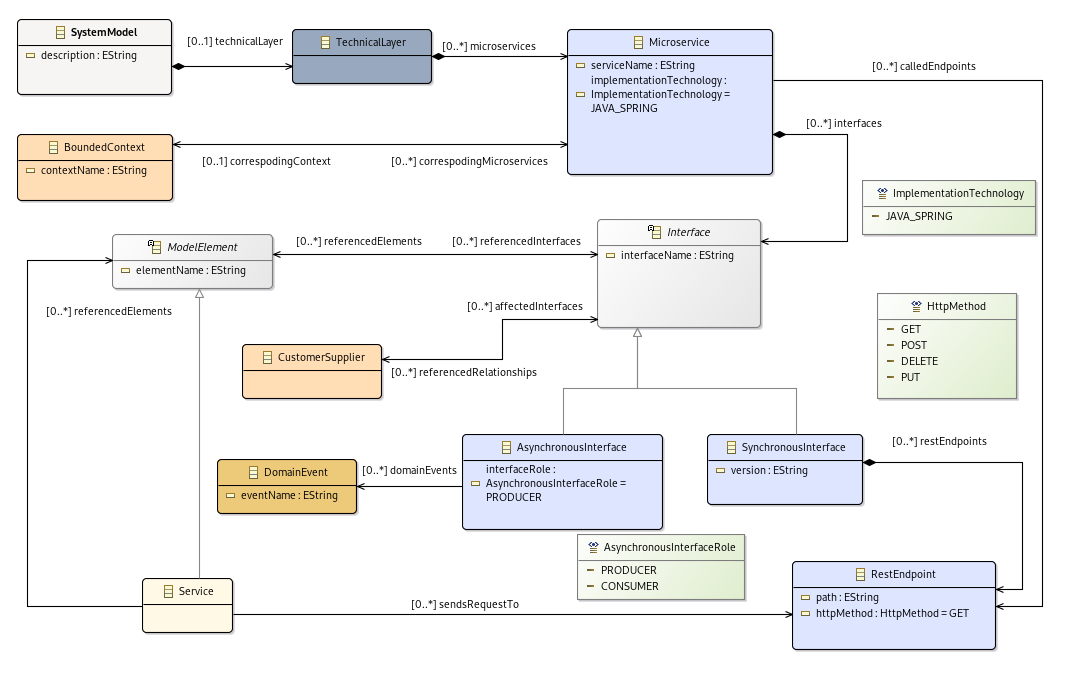
\includegraphics[width=\textwidth]{bilder/k4/5.png}
\caption{Metamodell - Fokus: Technische Schicht}
\end{figure}

Die technische Modellebene wird mit einer Klasse \glqq TechnicalLayer\grqq{} umgesetzt, welche die Microservices enthält. Die dazugehörige Klasse \glqq Microservice\grqq{} ist benannt und weiterhin mit einem Attribut vom Typ \glqq ImplementationTechnology\grqq{} versehen. Mögliche Implementierungstechnologien können so zukünftig hinzugefügt werden. Ein Objekt der Klasse Microservice besitzt beliebig viele \glqq Interfaces\grqq{}. Von dieser benannten abstrakten Klasse existieren weiterhin die Ableitungen \glqq AsynchronousInterface\grqq{} und \glqq SynchronousInterface\grqq{}. Asynchrone Schnittstellen sind dabei entweder Produzenten oder Konsumenten. Synchrone Schnittstellen sind demgegenüber versioniert und implementieren HTTP-Schnittstellen. Hier wird sich bewusst für eine Eingrenzung auf die Protokolle HTTP und das REST-Paradigma entschieden, da diese für synchrone Schnittstellen die relevantesten im Microservice-Kontext sind. Die zur synchronen Schnittstelle gehörigen REST-Endpunkte, modelliert durch eine Klasse \glqq RestEndpoint\grqq{}, besitzen einen Pfad sowie eine HTTP-Methode. Diese wird im dazugehörigen Enum spezifiziert. Bei der Konzeption der Implementierungsumsetzung der MDD-Bausteine wurde anfangs versucht, Gegenstücke zu diesen als eigenständige Klassen der technischen Schicht zu definieren. Jedoch stellte sich heraus, dass aufgrund des grundlegenden Konzepts des MDD, dem Erzeugen einer hohen Kohäsion zwischen Modellbausteinen und Umsetzung dieser, diese nicht zwingend benötigt werden. Dadurch hat eine Abwägung stattgefunden: Es wurde erwogen, ob aus Gründen der kognitiven Komplexität des Metamodells bestimmte Elemente explizit als Teil der Schicht definiert werden sollen.

Die alternative Überlegung war, ob auf diese Definition verzichtet werden sollte, obwohl Modellelemente in der technischen Abstraktionsebene implizit existieren. Entschieden wurde, auf die explizite Definition zu verzichten.

Die Klassen der technischen Schicht besitzen weiterhin verschiedene Assoziationen zu Klassen der fachlichen Schicht. So kann ein BoundedContext durch beliebig viele Microservices umgesetzt werden. Zwischen ModelElements und Interfaces können bidirektional beliebig viele Assoziationen existieren. Eine CustomerRelationship-Beziehung kann beliebig viele Schnittstellen betreffen. Ebenso kann eine Schnittstelle beliebig viele referenzieren. Dem AsynchronousInterface können verschiedene DomainEvents zugewiesen werden. Dies ist insbesondere im Prozess der Analyse der Problemdomäne eine wertvolle Assoziation.

Um den Zugriff auf REST-Endpunkte zu modellieren, wird einerseits eine Assoziation vom Microservice zum RestEndpoint eingeführt. Diese ist notwendig, um auf der Intermicroservice-Kommunikationsebene Architekturen zu entwerfen. Zusätzlich kann spezifiziert werden, wo im Service selbst ein Aufruf ausgelöst wird. Dafür wurde basierend auf dem MDD und somit der Richtlinie, Logik durch Services primär umzusetzen, dieses Aufrufen in der Klasse Service verortet.

%%%%%%%%%%%%%%%%%%%%%%%%%%%%%%%%%%%%%%%%%%%%%%%%%%%%%%%%%%%%%%%%%%%%%%%%%%%%%%%%%%%%%%%%%%%%%%%%%%%%%%%%%%%%%%%%%%%%
%			Infrastruktur
%%%%%%%%%%%%%%%%%%%%%%%%%%%%%%%%%%%%%%%%%%%%%%%%%%%%%%%%%%%%%%%%%%%%%%%%%%%%%%%%%%%%%%%%%%%%%%%%%%%%%%%%%%%%%%%%%%%%
\subsection{Modellierung der Infrastrukturellen Umgebung}

\begin{figure}[ht]
\centering
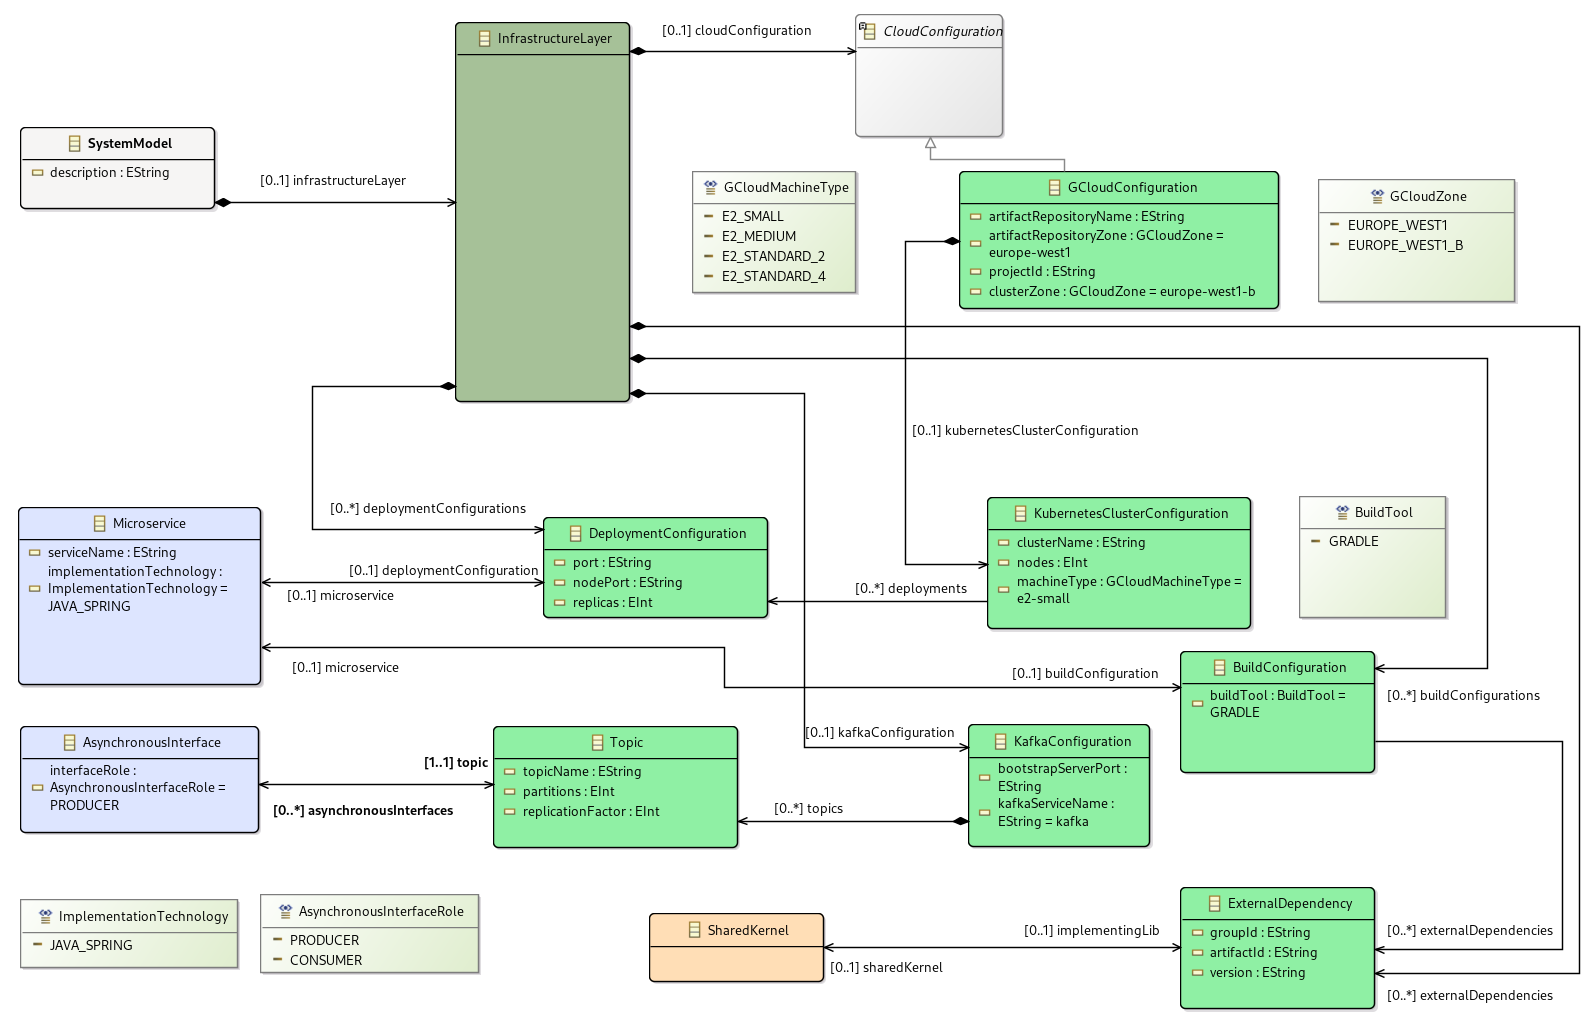
\includegraphics[width=\textwidth]{bilder/k4/6.png}
\caption{Metamodell - Fokus: Infrastrukturschicht}
\end{figure}

\newpage

Die Infrastrukturebene, umgesetzt durch die Klasse \glqq InfrastructureLayer\grqq{}, besitzt eine Konfiguration der Cloud-Umgebung. Diese wird als abstrakte Klasse \glqq CloudConfiguration\grqq{} entworfen, von der die \glqq GCloudConfiguration\grqq{} abgeleitet wird. Ergänzungen für AWS oder Azure würden dort ansetzen. Die GCloudConfiguration definiert GCP-spezifische, notwendige Eigenschaften. So definiert \glqq artifactRepositoryName\grqq{} und \glqq artifactRepositoryZone\grqq{} ein Ziel-Repository für Docker Images.

Das Attribut \glqq clusterZone\grqq{} definiert die Google-spezifische Region des Kubernetes-Clusters, welches durch die Klasse \glqq KubernetesClusterConfiguration\grqq{} modelliert wird. Diese wird außerdem als Teil der GCloudConfiguration modelliert. Bei der Kubernetes Konfiguration muss weiterhin bedacht werden, dass ein Kubernetes-Cluster Attribute besitzt, die unabhängig von dem Cloud-Anbieter sind. Jedoch gibt es auch welche die cloudspezifisch sind. Konkret wird hier noch ein Google-spezifischer Maschinentyp verwendet, welcher bei einer Erweiterung der Cloud Umgebungen abstrakter konzipiert werden müsste. Ebenso wird aktuell nur ein existierendes Cluster in der Cloud modelliert, da dies hinreichend für das Deployment einer Microservice-Architektur ist. Grundsätzlich möglich wären aber auch mehrere Cluster in einer Cloud-Umgebung.

Das Cluster referenziert weiterhin die Klasse \glqq DeploymentConfiguration\grqq{}. Diese beschreibt Deployment-Objekte in einem Kubernetes-Cluster. Modelliert werden diese als Teil der Infrastrukturschicht. Sie haben weiterhin eine bidirektionale Assoziation, welche Objekte der Klasse zu einem Microservice zuweisen können. Hier wurde darauf verzichtet das Konzept der Pods in das Metamodell mit aufzunehmen um die Komplexität zu reduzieren. Es wird daher festgelegt, dass jeder Service auf genau einem Pod, der genau einem Deployment zugewiesen ist, ausgeführt wird.

Symmetrisch zu der DeploymentConfiguration wurde die bidirektionale Assoziation für die Klasse \glqq BuildConfiguration\grqq{} und Microservice modelliert. Diese sind Teile der Infrastrukturschicht und gehen von einer Verwendung des Build-Tools Gradle aus. Andere Build-Tools wie z.B. Maven können in der dazugehörigen Enumeration \glqq BuildTool\grqq{} bei möglicher Erweiterung des Metamodells ergänzt werden. Die BuildConfiguration verweist auf die Klasse \glqq ExternalDependency\grqq, ebenfalls Teil des InfrastructureLayers. Diese besitzt eine auf das öffentliche Bibliotheksverzeichnis \glqq mvnrepository\grqq{} abgestimmte Attributierung. Eine weitere Relation zwischen ExternalDependency und SharedLib modelliert den Zusammenhang dieser.

Eine \glqq KafkaConfiguration\grqq{} definiert Port und Service-Name eines Kafka-Containers in der Cloud. Hier wurde sich gegen eine Abstraktion der asynchronen Kommunikationstechnologie entschieden, um die Komplexität des Metamodells nicht weiter zu erhöhen. Inwiefern eine Abstraktion verschiedener solcher Technologien überhaupt möglich wäre, wurde nicht näher betrachtet. Die KafkaConfiguration besitzt benannte Topics, welche von asynchronen Schnittstellen beschrieben oder konsumiert werden. Eine asynchrone Schnittstelle ist so modelliert, dass sie nur mit einem Topic interagiert. Weiterhin besitzt es die Attribute \glqq partitions\grqq{}, welches das Topic mit der angegebenen Zahl partitioniert, und \glqq replicationFactor\grqq{}, welches die Anzahl der Replikationen für Ausfälle definiert.


%%%%%%%%%%%%%%%%%%%%%%%%%%%%%%%%%%%%%%%%%%%%%%%%%%%%%%%%%%%%%%%%%%%%%%%%%%%%%%%%%%%%%%%%%%%%%%%%%%%%%%%%%%%%%%%%%%%%
%			Konkrete Syntax
%%%%%%%%%%%%%%%%%%%%%%%%%%%%%%%%%%%%%%%%%%%%%%%%%%%%%%%%%%%%%%%%%%%%%%%%%%%%%%%%%%%%%%%%%%%%%%%%%%%%%%%%%%%%%%%%%%%%
\newpage
\chapter{Entwicklung einer konkreten Syntax}

Mit Hilfe des Eclipse Modeling Frameworks und der Sirius-Erweiterung ist es möglich, spezifische Modelle zu konzeptionieren und zu visualisieren, die auf dem entwickelten Microservice-Metamodell basieren. Im Folgenden wird eine konkrete Syntax präsentiert und erörtert, wie diese erstellt wurde. Dabei wurde versucht, die Komplexität von Microservice-Architekturen durch verschiedene Modellsichten greifbarer zu machen, welche sich gegenseitig ergänzen.

Beginnend soll ein grundlegender, abstrakter Workflow skizziert werden, welcher die Modellierung einer Microservice-Architektur mit der DSL beschreibt. Dazu wird festgelegt, dass ein initiales Grundmodell vorhanden sein muss. Dieses muss alle notwendigen Wurzelklassen, wie zum Beispiel die Klasse \glqq System Model\grqq{}, beinhalten. Danach wird die Problemdomäne konzeptionell erfasst. Dies würde durch ein zuweisen der DDD-Konzepte, bzw. der Metamodellklassen der DomainModelLayer, umgesetzt werden. Dazu sollen im folgenden notwendige Darstellungen und Editoren entworfen werden. In einem nächsten Schritt, kann ein Modell mit einer technischen Schicht erweitert werden, welche die konkreten Dienste dazu modelliert. Abschließend soll eine dazu passende Infrastrukturschicht modelliert werden, die wiederum das bis zu diesem Schritt modellierte Modell ergänzt. Auch hierfür werden im folgenden Darstellungen und Editoren entworfen.

\begin{figure}[ht]
\centering
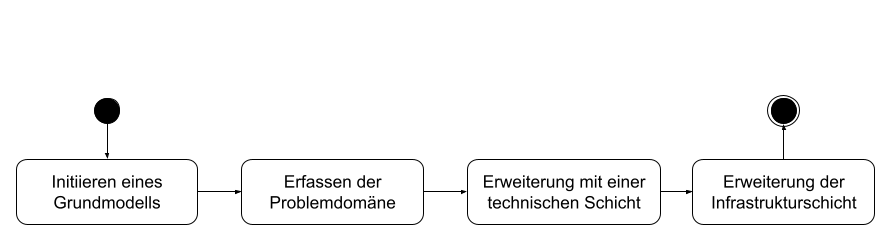
\includegraphics[width=\textwidth]{bilder/k5/workflow1.png}
\caption{Ein abstrakter Modellierungsworkflow für das Microservice-Metamodell}
\end{figure}


\newpage
\section{Entwurf des Editors}

Die verschiedenen Visualisierungen und Werkzeuge werden mit einer \glqq Sirius Viewpoint Specification\grqq{} umgesetzt. Grundlegend funktioniert dies analog zu den Methoden, die in der dieser Arbeit vorausgehenden Seminararbeit vorgestellt wurden \cite[S.11-13]{loeffler}.

Aufgrund der Komplexität des Metamodells ergeben sich grundlegende konzeptionelle Fragen, die vor der eigentlichen Umsetzung zu klären sind. Es hat sich gezeigt, dass der Versuch, allumfassende Modelldiagramme zu erstellen, kognitiv schwer nachvollziehbar war. Der ursprüngliche Ansatz, pro Schicht ein separates Diagramm zu verwenden, wurde daher verworfen. Stattdessen zielt die Neukonzeption der Diagramme darauf ab, einen effektiven Workflow zu unterstützen. Zudem soll der Einsatz verschachtelter Darstellungen, bei denen einzelne Grafiken als Elemente in übergeordneten Strukturen dienen, das Verständnis erleichtern und eine strukturierte Präsentation ermöglichen.

Zentral für den Entwurf sind verschiedene AQL-Ausdrücke, die genutzt werden, um Logik in der grafischen Oberfläche umzusetzen. So erweist sich die Umsetzung des Werkzeugs, das Microservices in der \glqq ContextRelationshipDescription\grqq{}, einem Diagramm welches die Beziehungen von BoundedContexts zueinander zeigt, erzeugt, als verhältnisweiße komplex:

\begin{lstlisting}[caption=Erzeugen eines Microservices als Border Node an einem Bounded Context]
//Precondition
aql:self.oclIsTypeOf(microserviceMetamodell::BoundedContext)

//Change Context to Right Container
aql:self.eContainer().eContainer().technicalLayer

//Setting the service name after creating the instance for the layer
aql:self.correspodingContext.contextName.toLower().concat('-service')

//Changing back to the container, the bounded context,
var:container
//and setting cotainer.correspondingMicroservices to the instance which was created before
var:instance
\end{lstlisting}

Dieser Ansatz musste öfters ähnlich angewandt werden. Grund hierfür ist die Entscheidung gegen Diagramme, welche nur die Schichtebene visualisieren. Dadurch muss an einigen Stellen auf hierarchisch höher liegende Container zugegriffen werden, um die passenden Objekte zu referenzieren. Weiterhin wird der Ansatz der typisierten Vorbedingung häufig genutzt.

Eine andere Art von Problematik ergibt sich bei der Darstellung durch rekursive Beziehungen von Elementen zu sich selbst. Dies soll am Beispiel der \glqq AggregateStructureDescription\grqq{}, welche die Struktur eines Aggregate visualisiert, verdeutlicht werden.

\newpage

\begin{figure}[ht]
\centering
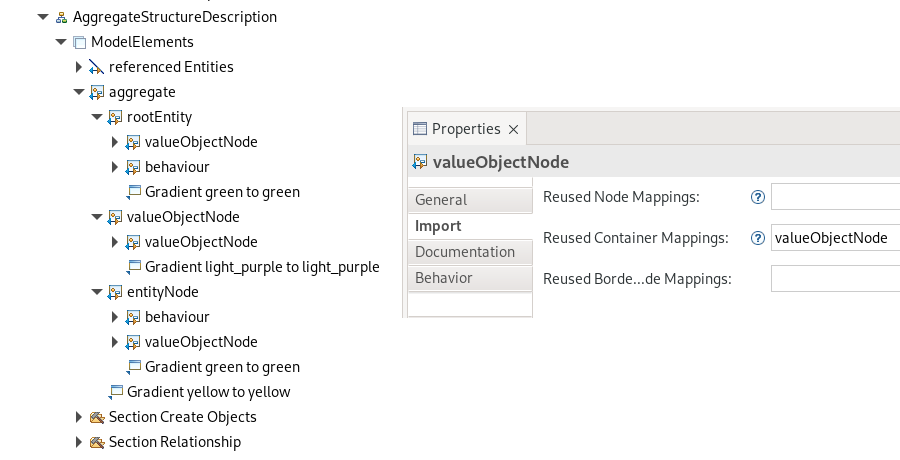
\includegraphics[width=0.7\textwidth]{bilder/k5/7.png}
\caption{Umsetzen von rekursiven Aufrufen durch das importieren von Nodes mit Sirius}
\end{figure}

Hier ist zu beachten, dass eine rekursive Beziehung, wie sie beispielsweise der ValueObjectNode aufweist, korrekt umgesetzt wird. Dazu muss der Node, der sich selbst enthält, sich selbst importieren, wie in der Abbildung zu sehen ist. Weiterhin stellt sich nun die Frage, ob eine Darstellung solcher rekursiven Beziehungen grundsätzlich sinnvoll ist.

\begin{figure}[ht]
\centering
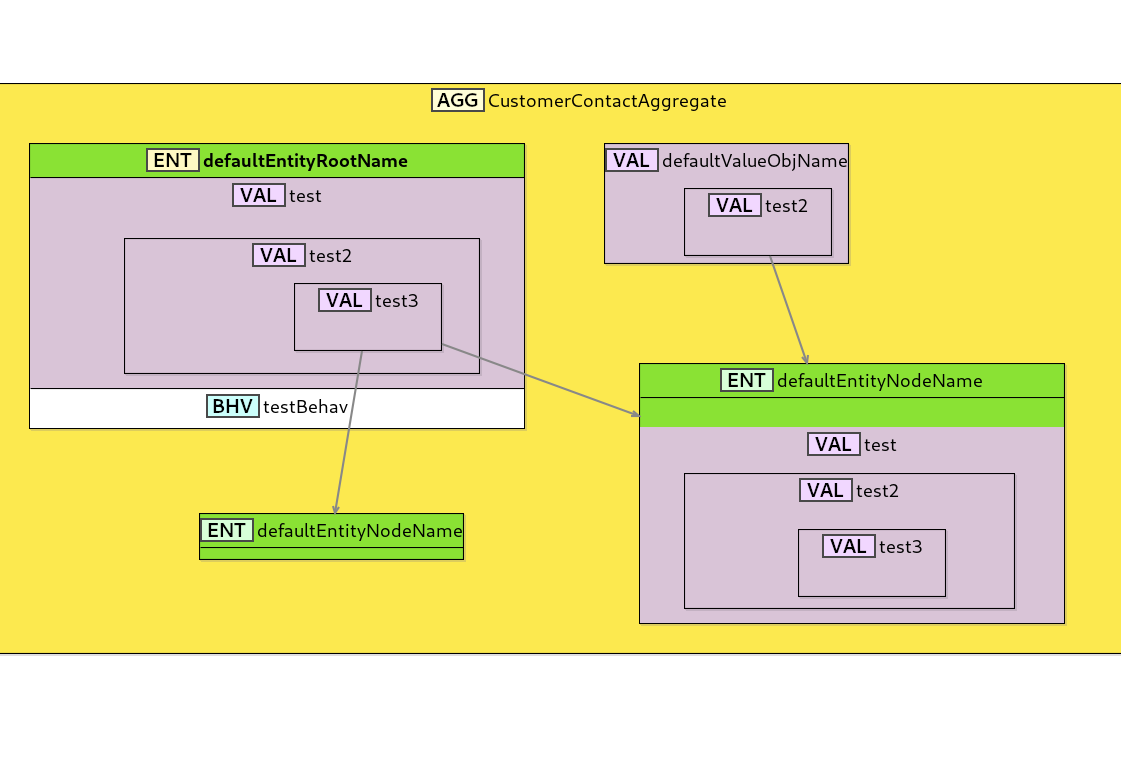
\includegraphics[width=0.8\textwidth]{bilder/k5/8.png}
\caption[Eine kognitiv anspruchsvolle Aggregate Visualisierung]{Eine kognitiv anspruchsvolle Aggregate Visualisierung - Hat ein Betrachter hier noch einen Mehrwert ?}
\end{figure}

Eine Modellierung von Klassenattributen in der Implementierung wurde bisher nicht berücksichtigt. Dies sollte im Rahmen der notwendigen Feinimplementierung händisch geschehen. Da außerdem auch andere EMF-Beschreibungsmodelle existieren, die für genau diese Aufgabe konzipiert wurden, wird die Entscheidung getroffen, keine Anpassung vorzunehmen und die Attributierung nicht konzeptionell in das Metamodell aufzunehmen. Fortschreitend werden für die Entity und das ValueObject keine feineren Strukturdiagramme entworfen. Konzeptionell würden diese jedoch symmetrisch zur AggregateStructureDescription umgesetzt werden.

%%%%%%%%%%%%%%%%%%%%%%%%%%%%%%%%%%%%%%%%%%%%%%%%%%%%%%%%%%%%%%%%%%%%%%%%%%%%%%%%%%%%%%%%%%%%%%%%%%%%%%%%%%%%%%%%%%%%
%			Diagramme
%%%%%%%%%%%%%%%%%%%%%%%%%%%%%%%%%%%%%%%%%%%%%%%%%%%%%%%%%%%%%%%%%%%%%%%%%%%%%%%%%%%%%%%%%%%%%%%%%%%%%%%%%%%%%%%%%%%%
\newpage
\section{Beschreibung der Diagramme}

\subsection{ContextRelationshipDescription}

Diese Darstellung zeigt die in einer DomainModelLayer vorhandenen BoundedContexts und ihre Beziehungen zueinander. Zweck des Diagramms ist die initiale Feststellung von Kontexten bei der Analyse einer Problemdomäne. Weiterhin können hier DomainModels und Microservices für einen Bounded Context erzeugt und implizit zugewiesen werden. Für eine Shared Kernel Beziehung, welche durch einen eigenen Container dargestellt wird, kann eine ExternalDependency ebenso erzeugt und implizit zugewiesen werden. Andere Beziehungstypen werden durch eine Auswahl im Eigenschaftsfenster mittels Radio-Buttons realisiert. Module können außerdem hier schon erzeugt werden, sofern einem BoundedContext ein DomainModel zugewiesen ist. Das Erzeugen eines Moduls in einem SharedKernel führt dabei zur Erstellung eines SharedModule.

\begin{figure}[ht]
\centering
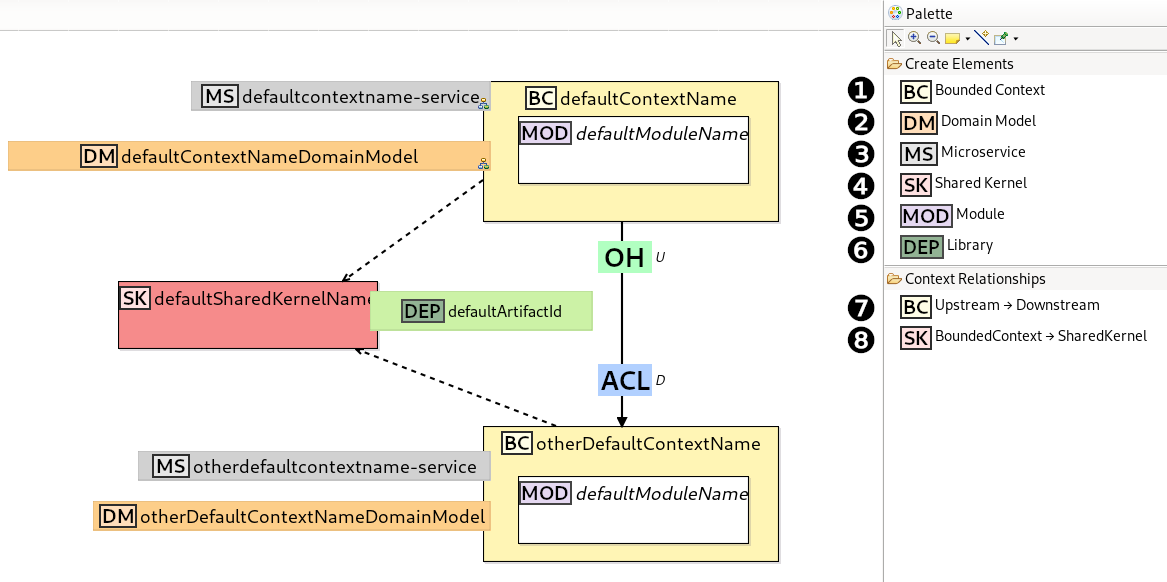
\includegraphics[width=\textwidth]{bilder/k5/1.png}
\caption{Editoransicht der ContextRelationshipDescription}
\end{figure}


\begin{table}[h]
\centering
\footnotesize
\begin{tabularx}{\textwidth}{|c|X|}
\hline
1 & Erzeugt ein BoundedContext. Namenskonvention: camelCase \\ \hline
2 & Erzeugt auf einem BoundedContext ein zugewiesenes DomainModel. Namenskonvention: camelCase \\ \hline
3 & Erzeugt auf einem BoundedContext ein zugewiesenen Microservice. Namenskonvention: kebap-case \\ \hline
4 & Erzeugt ein SharedKernel. Namenskonvention: camelCase \\ \hline
5 & Erzeugt auf einem BoundedContext oder SharedKernel ein (Shared)Module.\\ & Vorbedingung: Existierendes DomainModel. Namenskonvention: camelCase \\ \hline
6 & Erzeugt auf einem SharedKernel eine ExternalDependency.\\ & Namenskonvention: Abh. zu der Bezeichnung in mvnrepository \\ \hline
7 & Erzeugt Beziehung zwischen Quellkontext (Upstream) und Zielkontext (Downstream).\\ &  Nähere Typisierung im Eigenschaftsfenster \\ \hline
8 & Verbindet ein BoundedContext mit einem SharedKernel \\ \hline
\end{tabularx}
\caption{Legende - ContextRelationshipDescription}
\end{table}

\subsection{DomainModelDescription}

Die \glqq DomainModelDescription\grqq{} visualisiert ein DomainModel. Sie zeigt Module, die es enthält, sowie DomainEvents, die mit dem Modell assoziiert sind. Zudem stellt sie die verwendeten ModelElements dar und ermöglicht es dem Bearbeiter, diese nach Bedarf mit anderen Elementen des DomainModels zu verknüpfen. Außerdem visualisiert sie die in Entities und Aggregates enthaltenen Objekte.

\begin{figure}[ht]
\centering
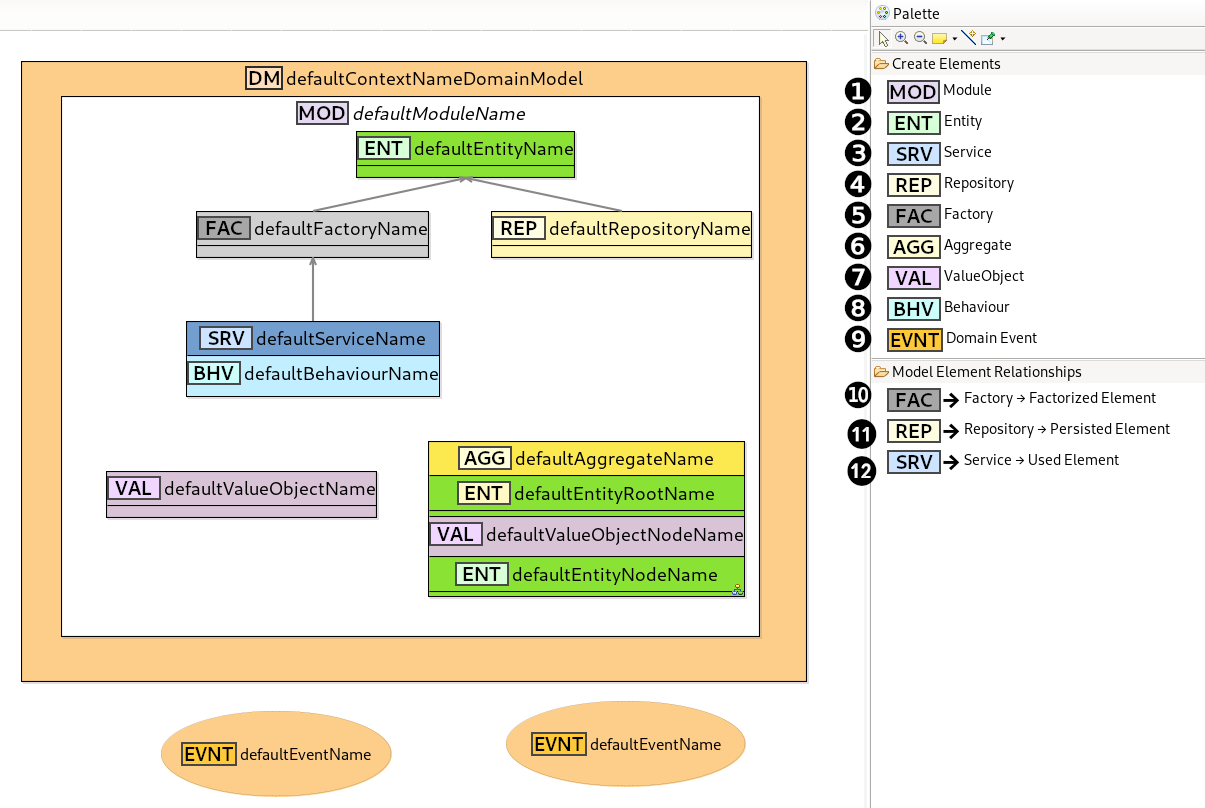
\includegraphics[width=\textwidth]{bilder/k5/2.png}
\caption{Editoransicht der DomainModelDescription}
\end{figure}


\begin{table}[h]
\centering
\footnotesize
\begin{tabularx}{\textwidth}{|c|X|}
\hline
1 & Erzeugt auf einem DomainModel ein enthaltenes Module. Namenskonvention: camelCase \\ \hline
2 & Erzeugt auf einem Module eine enthaltene Entity. Namenskonvention: camelCase \\ \hline
3 & Erzeugt auf einem Module einen enthaltenen Service. Namenskonvention: camelCase \\ \hline
4 & Erzeugt auf einem Module ein enthaltenes Repository. Namenskonvention: camelCase \\ \hline
5 & Erzeugt auf einem Module eine enthaltene Factory. Namenskonvention: camelCase \\ \hline
6 & Erzeugt auf einem Module ein enthaltenes Aggregate. Namenskonvention: camelCase \\ \hline
7 & Erzeugt auf einem Module ein enthaltenes ValueObject. Namenskonvention: camelCase \\ \hline
8 & Erzeugt auf geeigneten ModelElements ein Behaviour. Namenskonvention: camelCase \\ & Beim Repository zusätzlich: JPA konformer Funktionsname \\ \hline
9 & Erzeugt außerhalb des DomainModels ein zu diesem assoziiertes Event. Namenskonvention: keine \\ \hline
10 & Weist einer Factory ein Factorizable Element zu. \\ \hline
11 & Weist einem Repository ein Persistable Element zu. \\ \hline
12 & Weist einem Service ein Element zu. \\ \hline
\end{tabularx}
\caption{Legende - DomainModelDescription}
\end{table}

\newpage
\subsection{AggregateStructureDescription}

Um die kognitive Last, die durch komplexe Aggregates in der DomainModelDescription entstehen kann, zu reduzieren, wird eine AggregateStructureDescription genutzt. Diese spezialisiert sich auf die Darstellung der nach dem Metamodell verschachtelbaren Struktur. Diese wurde, wie bereits erläutert, zwar konzipiert, jedoch ist ihr Mehrwert diskutabel.

\begin{figure}[ht]
\centering
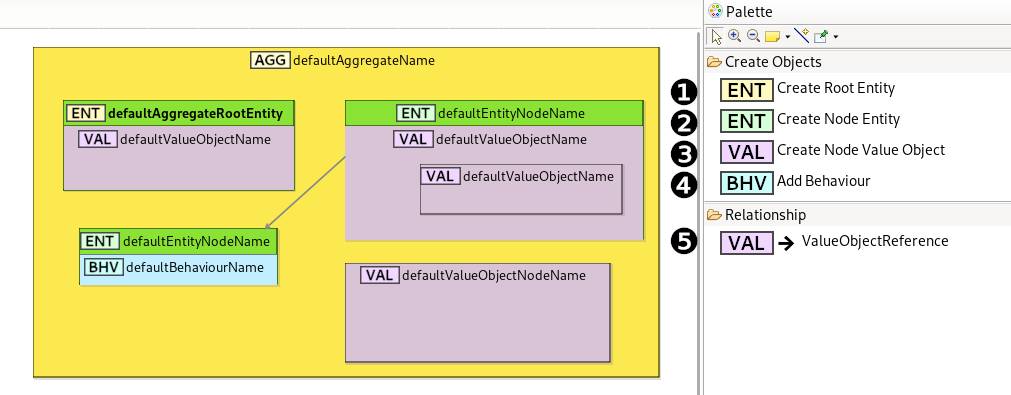
\includegraphics[width=\textwidth]{bilder/k5/3.png}
\caption{Editoransicht der AggregateStructureDescription}
\end{figure}


\begin{table}[h]
\centering
\footnotesize
\begin{tabularx}{\textwidth}{|c|X|}
\hline
1 & Erzeugt (eimalig) auf einem Aggregate eine dazugehörende EntityNode als Wurzel. Namenskonvention: camelCase \\ \hline
2 & Erzeugt auf einem Aggregate eine EntityNode als Blatt. Namenskonvention: camelCase \\ \hline
3 & Erzeugt auf einem Aggregate, einer Entity oder einem ValueObject ein enthaltenes ValueObject.\\ & Namenskonvention: camelCase \\ \hline
4 & Erzeugt auf einer Entity ein Behaviour. Namenskonvention: camelCase \\ \hline
5 & Weist einem ValueObject eine referenzierte Entity zu \\ \hline
\end{tabularx}
\caption{Legende - AggregateStructureDescription}
\end{table}

\newpage
\subsection{MicroserviceCommunicationDescription}

Die \glqq MicroserviceCommunicationDescription\grqq{} zeigt die Microservices in der technischen Schicht. Interfaces können hier betrachtet und verwaltet werden. Durch die zusätzliche Visualisierung der DomainEvents, die dem Microservice zugehörigen DomainModel zugewiesen sind, kann der Betrachter sich bei der Modellierung an diesen orientieren, um AsynchronousInterface Objekte zu verorten. SynchronousInterfaces können hier RestEndpoints zugewiesen werden. AsynchronousInterfaces können weiterhin Topics zugewiesen werden. Mit Werkzeugen zum Verbinden der Kommunikationsteilnehmer kann hier somit eine vollständige Übersicht der Kommunikationsabläufe in einer Microservice-Architektur umgesetzt werden.

\begin{figure}[ht]
\centering
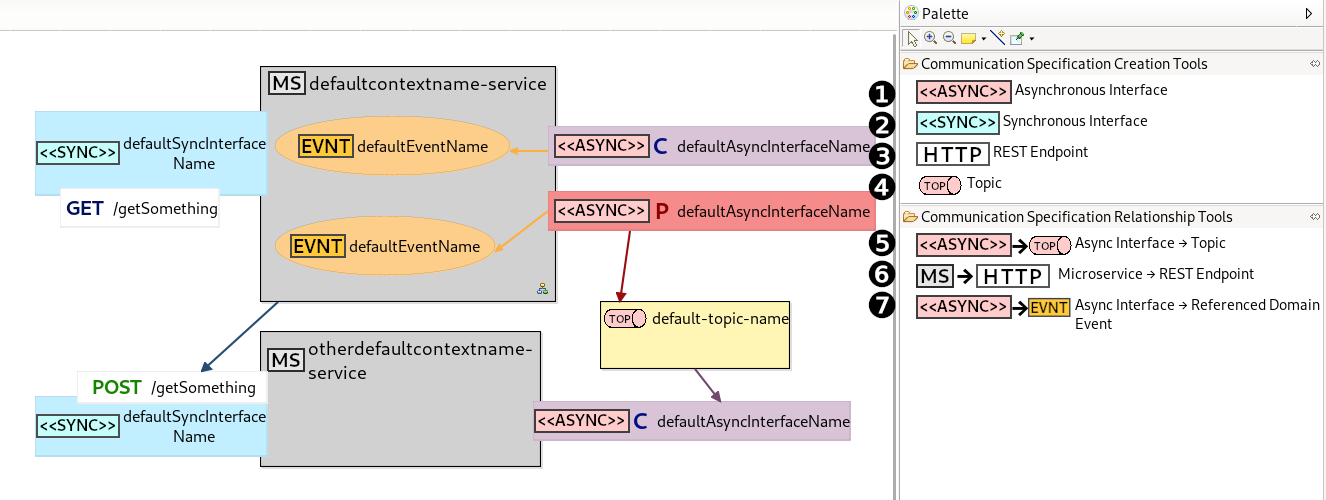
\includegraphics[width=\textwidth]{bilder/k5/4.png}
\caption{Editoransicht der MicroserviceCommunicationDescription}
\end{figure}


\begin{table}[h]
\centering
\footnotesize
\begin{tabularx}{\textwidth}{|c|X|}
\hline
1 & Erzeugt auf einem Microservice ein zugewiesenes AsynchronousInterface. Namenskonvention: camelCase   \\ \hline
2 & Erzeugt auf einem Microservice ein zugewiesenes SynchronousInterface. Namenskonvention: camelCase \\ \hline
3 & Erzeugt auf einem SynchronousInterface einen zugewiesenen RestEndpoint. Namenskonvention: "/" + camelCase \\ \hline
4 & Erzeugt ein neues Topic. Setzt existierende KafkaConfiguration voraus. Namenskonvention: kebap-case\\ \hline
5 & Weist einem AsynchronousInterface ein Topic zu.\\ & Datenflussrichtung wird implizit aus Rolle der Schnittstelle bestimmt. \\ \hline
6 & Weist einem Microservice einen zu aufrufenden RestEndpoint zu. \\ \hline
7 & Weist einem AsynchronousInterface ein Event zu. \\ \hline
\end{tabularx}
\caption{Legende - MicroserviceCommunicationDescription}
\end{table}

\newpage
\subsection{MicroserviceInterfaceDescription}

Die folgende \glqq MicroserviceInterfaceDescription\grqq{} dient der Darstellung und Verwaltung der Kommunikation und deren Ursprung auf Service-Ebene. Daher werden Relationen aus dem DomainModel ausgeblendet. Zusätzlich werden Interfaces des Dienstes und RestEndpoints anderer Dienste, die dem Microservice zugewiesen sind, visualisiert. Das Anlegen und Zuweisen dieser externen Schnittstellen wird nur in der MicroserviceCommunicationDescription umgesetzt, um die kognitive Last dieser Beschreibung zu reduzieren.

\begin{figure}[ht]
\centering
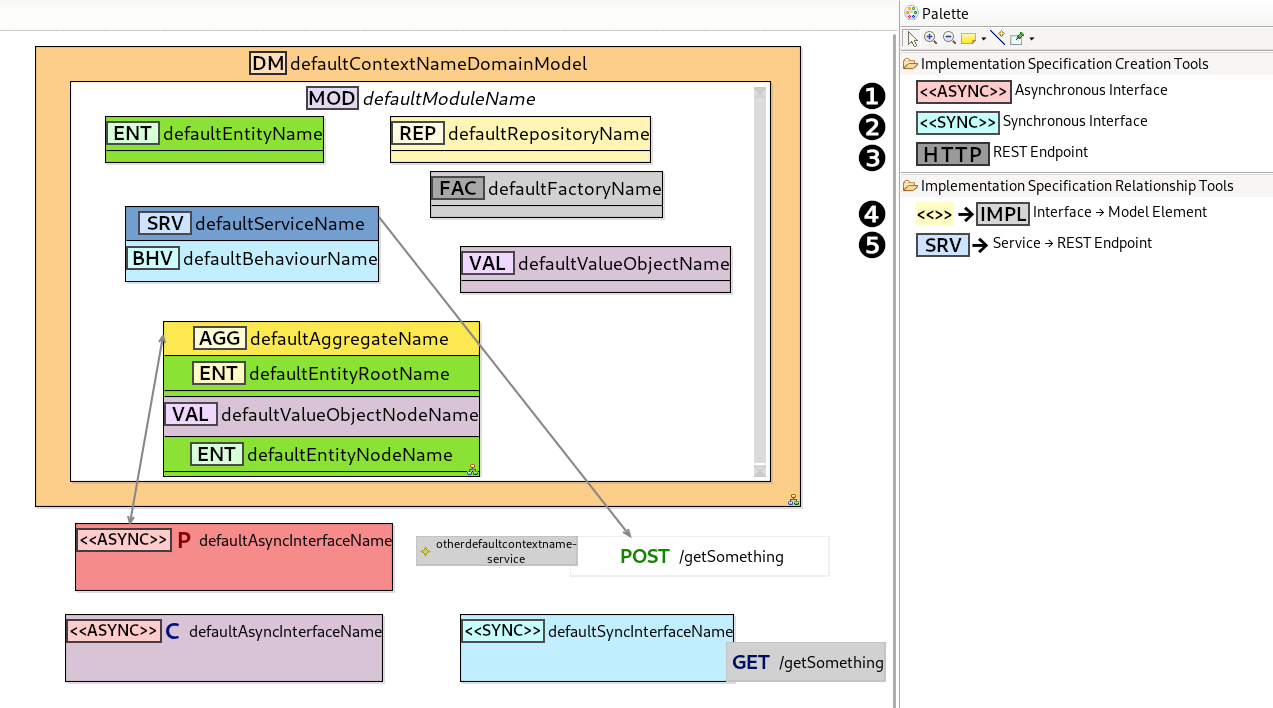
\includegraphics[width=\textwidth]{bilder/k5/5.png}
\caption{Editoransicht der MicroserviceInterfaceDescription}
\end{figure}

\begin{table}[h]
\centering
\footnotesize
\begin{tabularx}{\textwidth}{|c|X|}
\hline
1 & Erzeugt ein AsynchronousInterface. Namenskonvention: camelCase\\ \hline
2 & Erzeugt ein SynchronousInterface. Namenskonvention: camelCase \\ \hline
3 & Erzeugt auf einem SynchronousInterface einen RestEndpoint.\\ & Namenskonvention: "/" + camelCase\\ \hline
4 & Weist einem Interface referenzierte ModelElements zu. \\ \hline
5 & Weist einem Service einen externen, zu aufrufenden RestEndpoint zu. \\ \hline
\end{tabularx}
\caption{Legende - MicroserviceInterfaceDescription}
\end{table}

\newpage
\subsection{InfrastructureOverviewDescription}

Schließlich wird in der \glqq InfrastructureOverviewDescription\grqq{} die Infrastrukturschicht dargestellt. Hier werden vor allem Konfigurationen angelegt und diese den existierenden Microservices zugewiesen. Weiterhin werden zusätzliche modellierte Abhängigkeiten dargestellt.

\begin{figure}[ht]
\centering
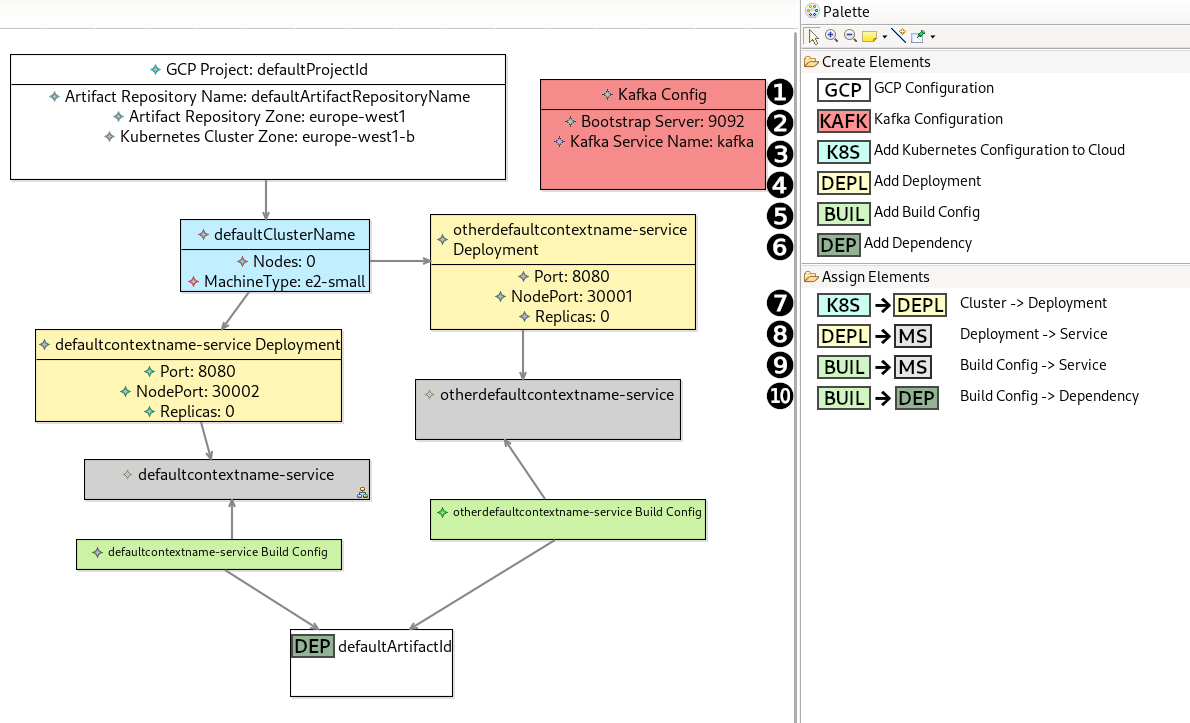
\includegraphics[width=\textwidth]{bilder/k5/6.png}
\caption{Editoransicht der InfrastructureOverviewDescription}
\end{figure}

\begin{table}[h]
\centering
\footnotesize
\begin{tabularx}{\textwidth}{|c|X|}
\hline
1 & Erzeugt eine GCloudConfiguration. Namenskonvention: Der GCP zu entnehmen, kebap-case \\ \hline
2 & Erzeugt eine KafkaConfiguration. Namenskonvention: kebap-case \\ \hline
3 & Erzeugt eine KubernetesClusterConfiguration. Namenskonvention: kebap-case \\ \hline
4 & Erzeugt eine DeploymentConfiguration. Namenskonvention: Generiert \\ \hline
5 & Erzeugt eine BuildConfiguration. Namenskonvention: Generiert \\ \hline
6 & Erzeugt eine ExternalDependency. Namenskonvention: Äquivalent zur Bennenung in mvnrepository \\ \hline
7 & Weist einer KubernetesClusterConfiguration DeploymentConfigurations zu. \\ \hline
8 & Weist einer DeploymentConfiguration einen Service zu. \\ \hline
9 & Weist einer BuildConfiguration einen Service zu. \\ \hline
10 & Weist einer BuildConfiguration eine Dependency zu. \\ \hline
\end{tabularx}
\caption{Legende - InfrastructureOverviewDescription}
\end{table}

\newpage

\section{Konkretisierung des Modellierungsworkflows}

Auf Basis des abstrakten Modellierungsworkflows wird nun ein konkreter Workflow, der den konzipierten Editor und die dazugehörige konkrete Syntax verwendet, definiert. Dazu kann beginnend eine dem Quellcodeverzeichnis beiliegende Modellvorlage \cite{mustermodell} verwendet werden. Alternativ können die notwendigen Klassen, die in Abbildung 5.10 aufgezählt werden, händisch in ein leeres EMF-Modell eingefügt werden. Der Schritt des Erfassens der Problemdomäne erfolgt durch das sequenzielle Anlegen der ContextRelationshipDescription, der DomainModelDescriptions (je DomainModel) und der AggregateStructureDescriptions. Darauf folgt die Konzeption der technischen Schicht mittels MicroserviceCommunicationDescription und MicroserviceInterfaceDescription (je Microservice). Abschließend wird mit der InfrastructureOverviewDescription die nötige Infrastruktur modelliert.

\begin{figure}[ht]
\centering
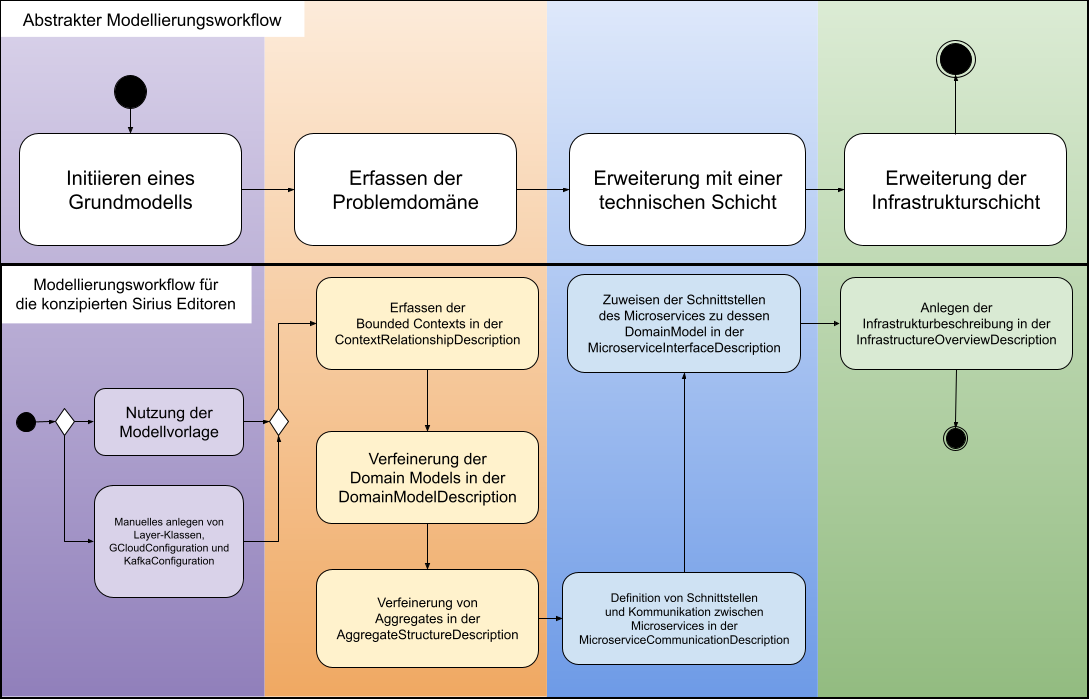
\includegraphics[width=\textwidth]{bilder/k5/workflow2.png}
\caption{Abbildung des abstrakten Modellierungsworkflows auf einem für diesen Editor angepassten Workflow}
\end{figure}
